\documentclass[12pt, a4paper]{article}
\usepackage[utf8]{inputenc}
\usepackage[T1]{fontenc}
\usepackage{mathpazo} 
\usepackage{amsmath, amssymb} 
\usepackage{algorithm}
\usepackage{algpseudocode}
\usepackage{graphicx} 
\usepackage{booktabs} 
\usepackage{float}


\usepackage{setspace}
\doublespacing

\usepackage{geometry} 
\geometry{margin=1in}

\usepackage[american]{babel} 
\usepackage{csquotes} 
\usepackage[backend=biber, style=apa, natbib=true]{biblatex}
\addbibresource{references.bib}

\usepackage[colorlinks=true, linkcolor=blue, citecolor=blue, urlcolor=blue]{hyperref}

% ---------------------------------------------------------
% Note: The \title and \author commands have been removed 
% as a designated title page will be attached separately.
% ---------------------------------------------------------

\begin{document}

% --- Summary Page ---
\begin{abstract}
    \thispagestyle{plain}
    This study developed an inference framework to realistically reproduce social contact networks—a critical element in infectious disease outbreak simulations—using the POLYMOD dataset.
    To overcome the limitations of conventional SIR models, which assume a homogeneous population, we proposed “Model 1,” which accounts for heterogeneity in individual sociability, and “Model 2B,” which explicitly incorporates cohort structures within educational institutions and multigenerational mixing within households.
    For statistical inference, to avoid the difficulty of likelihood calculation—a challenge in complex network models—we adopted an MCMC method using Synthetic Likelihood, thereby achieving stable inference in a high-dimensional parameter space.
    Simulation results revealed that while the presence of educational cohorts and hub individuals dramatically accelerates initial transmission, targeted interventions such as school closures nonlinearly suppress the epidemic peak (a 12.3\% reduction in Model 2B).
    This framework provides a powerful and extensible foundation for evaluating public health interventions with greater precision, taking into account future behavioral changes and the risk of contact substitution.
\end{abstract}
\newpage

% --- Table of Contents ---
\tableofcontents 
\newpage

% 1. Introduction
\section{Introduction}

Mathematical modeling of infectious diseases has become an indispensable tool for public health decision-making and outbreak forecasting.
Traditional compartmental models, such as the Susceptible-Infected-Recovered (SIR) framework, have historically relied on the assumption of homogeneous mixing, where every individual in a population has an equal probability of contacting any other individual.
However, recent empirical evidence and the global experience of the COVID-19 pandemic have clearly demonstrated that human interaction patterns are far from uniform.
\textcite{britton2025improving} argue that neglecting the inherent heterogeneity in social contacts can lead to significant biases in estimating the basic reproduction number ($R_0$) and the final epidemic size.
Therefore, incorporating realistic contact structures through network-based modeling is essential for accurately capturing the dynamics of disease transmission.

The foundation for constructing such realistic models lies in the empirical study of social mixing patterns.
The landmark POLYMOD study provided the first large-scale, population-based dataset on social contacts across eight European countries, revealing consistent patterns of age-dependent mixing and household clustering \parencite{mossong2008social}.
Since then, these contact matrices have been widely used to project transmission dynamics in various global settings, including low- and middle-income countries \parencite{prem2017projecting}.
Despite the richness of these survey-based data, a significant challenge remains in "reverse-engineering" these observed contact frequencies into a generative network model that can be used for high resolution stochastic simulations.

From a statistical perspective, inferring the underlying parameters of a contact network from survey data presents a formidable challenge.
Because the likelihood function for complex network-based epidemic models is often analytically intractable or computationally prohibitive, standard Maximum Likelihood Estimation (MLE) is frequently inapplicable \parencite{mckinley2009inference}.
Recent advancements in computational statistics, particularly Likelihood-Free Inference (LFI) and Synthetic Likelihood methods, have opened new avenues for parameter estimation in high-dimensional settings \parencite{ong2018likelihoodfree}.
By leveraging summary statistics that represent key network properties, these methods allow for the robust calibration of generative models without the need for an explicit likelihood function \parencite{picchini2023sequentially}.

The primary objective of this thesis is to develop a robust inference framework that reproduces the contact patterns observed in the POLYMOD dataset.
Specifically, we aim to estimate the "rules" or parameters that govern human connections and validate the resulting model through a synthetic population approach.
By reconstructing a structured contact network that explicitly accounts for sociability variance and school-based cohorts, we evaluate the effectiveness of targeted public health interventions, such as school closures.
This research bridges the gap between empirical contact surveys and generative network modeling, providing a scalable foundation for simulating realistic outbreak scenarios and evaluating the non-linear impacts of behavioral shifts.

The remainder of this thesis is organized as follows.
Section 2 describes the POLYMOD dataset and the data cleaning process.
Section 3 details the formulation of the network model and the Synthetic Likelihood MCMC inference pipeline.
Section 4 presents the results of the epidemic simulations and compares the effectiveness of different intervention strategies.
Finally, Section 5 discusses the implications of our findings, acknowledges limitations such as contact substitution, and outlines directions for future work.

% 2. Data
\section{Data}
\label{sec:data}

\subsection{The POLYMOD Contact Survey}
\label{subsec:polymod_intro}
The empirical foundation of this study relies on the POLYMOD dataset, a large-scale prospective survey of social mixing patterns conducted across eight European countries \parencite{mossong2008social}.
The survey was designed to quantify the nature of social interactions relevant to the transmission of respiratory and close-contact infectious diseases.
A total of 7,290 participants recorded their daily social interactions using a standardized paper-diary methodology \parencite{mossong2008social}.

The raw dataset fundamentally consists of two levels of information: participant-level data and contact-level data.
For each recorded contact, the diaries captured detailed characteristics, including the estimated age and gender of the contacted individual, the location of the interaction, the duration and frequency of the contact, and whether physical skin-to-skin contact occurred \parencite{mossong2008social}.
This rich multidimensional data provides the essential structure required to infer human contact networks and accurately simulate epidemic dynamics.

The survey covers eight European countries: Belgium, Germany, Finland, Great Britain, Italy, Luxembourg, the Netherlands, and Poland.
Participants were recruited from a broad demographic spectrum, ensuring that the collected contact patterns represent a diverse range of socio-economic and cultural contexts.
The robustness and cross-national consistency of the mixing patterns identified in POLYMOD have been further validated by subsequent large-scale modeling efforts.
Specifically, \textcite{prem2017projecting} and \textcite{mistry2021inferring} utilized the original POLYMOD matrices to construct and project synthetic contact matrices for diverse global settings beyond the original European context.
These studies underscore that while macroscopic mixing patterns vary across countries, the setting-specific contact probabilities captured by POLYMOD remain a gold standard for projecting transmission dynamics in a global context when combined with local demographic data.

\subsection{Data Cleaning and Preprocessing}
\label{subsec:data_cleaning}
To prepare the raw diary data for computational network inference, a series of systematic data cleaning and deterministic imputation procedures were applied. 
When exact ages of contacted individuals (\texttt{cnt\_age\_exact}) were not provided, the contact age (\texttt{cnt\_age}) was estimated as the midpoint between the recorded minimum and maximum estimated ages.
If only the minimum or maximum boundary was recorded, the available boundary value was utilized.

Missing values in key categorical variables were handled deterministically based on logical baselines: missing physical contact flags were replaced with a default indicating no physical contact, while unrecorded contact frequencies and durations were imputed with the lowest respective default categories.
Furthermore, individual location flags were consolidated into a single categorical variable (\texttt{location\_category}), classifying each interaction into primary settings such as School, Work, Home, Transport, Leisure, or Other.

Because the participants represent the core vertices (nodes) of the subsequent contact network models, any participant records with missing age (\texttt{part\_age}) or gender (\texttt{part\_gender}) were strictly excluded from the dataset.
Specifically, missing values accounted for approximately 0.12\% of the contact age and 1.39\% of the contact gender across all recorded interactions.
To address this, stochastic statistical imputation was performed for these missing attributes of the contacted individuals. 
Missing contact ages were imputed by constructing a reference pool grouped by the participant's age and the contact location category.
A value was then randomly sampled from the corresponding pool's empirical distribution.
If no corresponding reference pool existed, the participant's own age was assumed.
Similarly, missing contact genders were randomly drawn based on the overall probability distribution of contact genders within the dataset.


\subsection{Exploratory Data Analysis (EDA)}
\label{subsec:eda}

Prior to the construction of generative network models, an exploratory analysis was performed on the cleaned POLYMOD dataset.
This analysis aims to identify the fundamental structural characteristics and systemic biases inherent in human social mixing.

\subsubsection{Participant Demographics}
The foundation of any contact network is the demographic composition of its constituent nodes.
Figure \ref{fig:eda_demographics} illustrates the age distribution and gender ratio of the sampled survey participants.
The gender ratio is approximately balanced, with females comprising 52.5\% of the sample.
The age distribution features a prominent concentration of individuals between 10 and 20 years old, followed by a gradual decline in older age cohorts.
These empirical attributes directly inform the nodal characteristics required for the subsequent synthetic network generation.

\begin{figure}[H]
    \centering
    \begin{minipage}{0.48\textwidth}
        \centering
        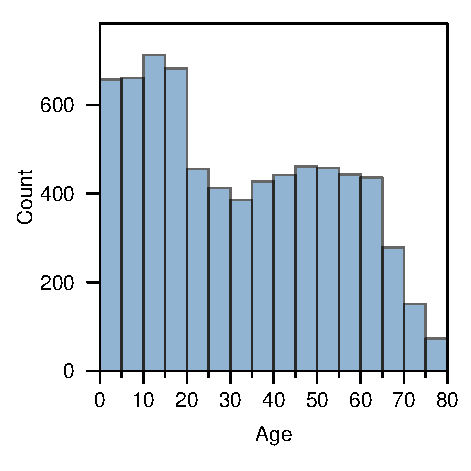
\includegraphics[width=\linewidth]{figures/02_Data/polymod_age_distribution.pdf}
    \end{minipage}\hfill
    \begin{minipage}{0.48\textwidth}
        \centering
        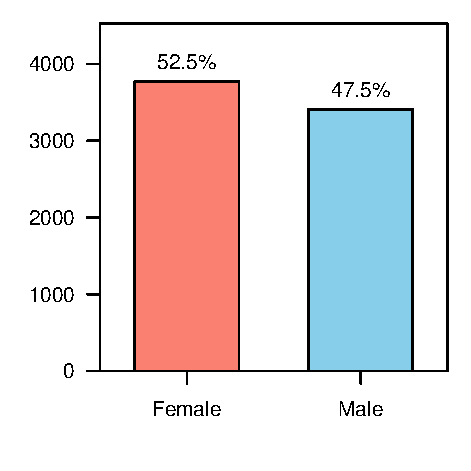
\includegraphics[width=\linewidth]{figures/02_Data/polymod_gender_ratio.pdf}
    \end{minipage}
    \caption{Participant demographics of the cleaned POLYMOD dataset. The left panel shows the age distribution with 5-year intervals, and the right panel displays the overall gender ratio.}
    \label{fig:eda_demographics}
\end{figure}

\subsubsection{Macroscopic Mixing Patterns}
Beyond individual attributes, the macroscopic volume and preference of interactions are captured by the contact matrix.
As visualized in Figure \ref{fig:eda_matrix}, the empirical data reveals a striking concentration of contacts along the main diagonal.
This intense diagonal band confirms the presence of strong age assortativity, indicating a universal human tendency to interact primarily with peers of a similar age.
Notably, the intensity of this assortative mixing is most pronounced among adolescents and young adults, reflecting the high-density contact environments characteristic of these life stages.
This concentrated activity among youths serves as a critical focal point for potential epidemic acceleration, which will be further explored in Chapter 4.

\begin{figure}[H]
    \centering
    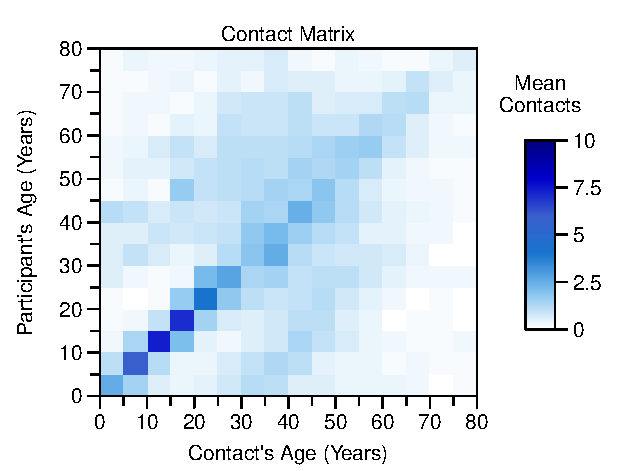
\includegraphics{figures/02_Data/polymod_contact_matrix_legend.pdf}
    \caption{Empirical contact matrix demonstrating strong age-assortative mixing. The darker blue cells along the diagonal indicate higher frequencies of interaction between individuals of the same age group.}
    \label{fig:eda_matrix}
\end{figure}

\subsubsection{Context-Specific Mixing Mechanisms}
While the macroscopic matrix highlights overall assortativity, disaggregating the contacts by location reveals distinct, context-specific mixing rules.
Figure \ref{fig:eda_location} presents the probability density of the absolute age difference between contacting pairs across four primary settings: Home, School, Work, and Leisure.
The school environment is characterized by an extreme, singular spike at an age difference of zero, demonstrating a rigid, highly stratified cohort structure.
Conversely, interactions within the home exhibit a bimodal distribution.
This bimodal shape consists of a primary peak at zero age difference, representing interactions between siblings or spouses, and a broader secondary peak around 30 years, representing inter-generational interactions between parents and children.
These empirical observations conclusively demonstrate that social networks are governed by multiple, overlapping spatial rules rather than a single homogeneous mixing parameter.
Consequently, capturing these dual mechanisms---the localized institutional clustering of schools and the broader inter-generational bridges of households---provides the foundational empirical justification for the mixture density architecture proposed in Model 2B.

\begin{figure}[H]
    \centering
    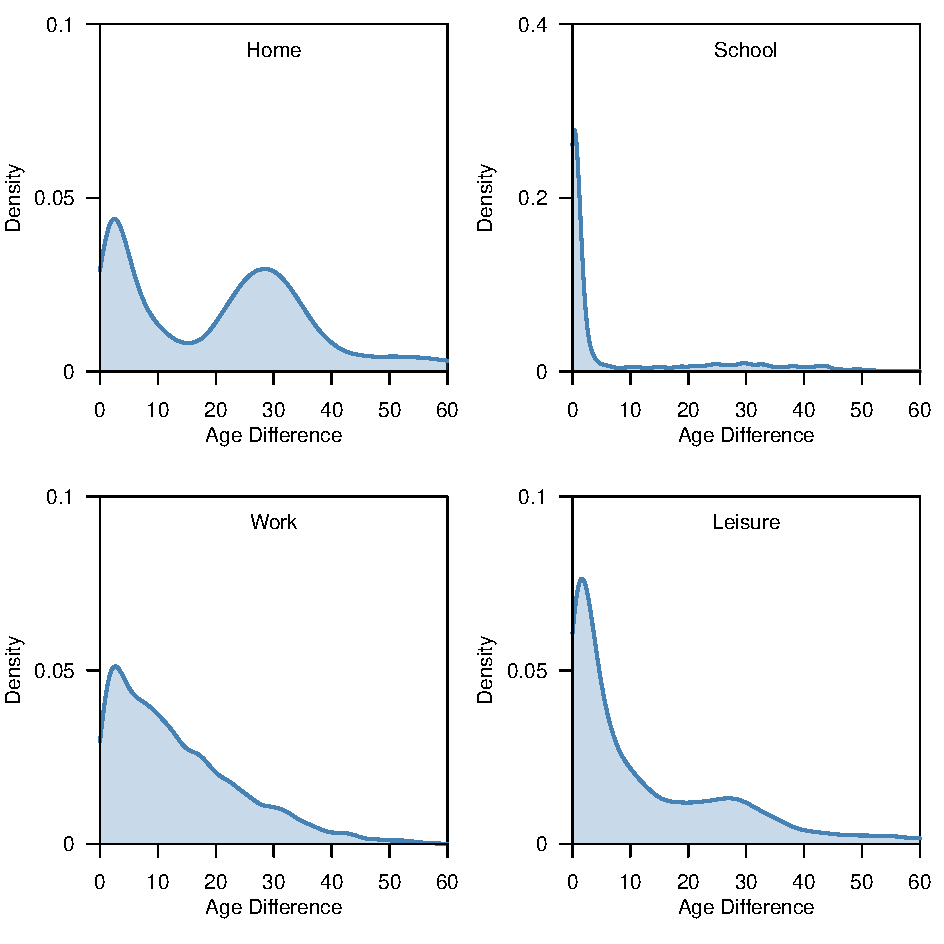
\includegraphics{figures/02_Data/polymod_agediff_location.pdf}
    \caption{Probability density of absolute age differences by contact location. The strict zero-difference spike in schools contrasts sharply with the bimodal (peer and inter-generational) distribution observed in households.}
    \label{fig:eda_location}
\end{figure}

\subsection{Population Sampling and Node Definition}
\label{subsec:sampling}
To bridge the gap between empirical data and computational simulation, we utilize a two-tier sampling strategy based on the cleaned POLYMOD distributions.
For the parameter inference stage (Section \ref{sec:inference}), a subset of $N = 1000$ unique participants was drawn using random sampling without replacement.
This reduced scale is mathematically necessary to manage the significant computational cost of the multi-stage Adaptive MCMC algorithm while preserving sufficient demographic heterogeneity.
For the subsequent large-scale epidemic simulations (Section \ref{sec:epidemic_model}), we expanded the node set to $N = 10,000$ individuals.
This larger synthetic population was sampled based on the Year 2000 European demographic distribution, ensuring that the infectious disease dynamics reflect a realistic societal scale.
Each node in these synthetic populations is assigned the age and gender attributes from the corresponding empirical records, grounding our simulations in the actual sociological landscape captured by the survey.

% 3. Network Model
\section{Network Model}
\label{sec:network_model}
% ==========================================
% file: sections/03_Methods/3_1_NetworkModel.tex
% ==========================================
To simulate the transmission dynamics of infectious diseases, we formalize the synthetic population as an undirected random graph $G = (V, E)$. Here, $V = \{v_1, v_2, \dots, v_n\}$ denotes the set of individuals (nodes), and $E$ represents the set of social contacts (edges) capable of facilitating disease transmission.
Let $N = |V|$ be the total population size.
Each node $v_i \in V$ is associated with a vector of demographic attributes $X_i = \{A_i, G_i\}$, where $A_i$ represents the continuous age of the individual and $G_i \in \{\text{Male}, \text{Female}\}$ represents their gender, derived directly from the empirical distributions of the POLYMOD dataset.
The formation of an edge between any two individuals $i$ and $j$ is treated as an independent conditional Bernoulli trial with probability $P_{ij} = P(A_{ij}=1 | X_i, X_j)$, where $A$ is the adjacency matrix of the network.
The functional form of $P_{ij}$ defines the structural complexity of the following proposed models.

\subsection{Model}

\subsubsection{Model 1: Baseline Demographic Model}
As a foundational structure, Model 1 incorporates basic demographic homophily alongside individual-level heterogeneity in sociability.
Rather than relying on complex, context-dependent attributes such as specific contact locations, this baseline model strictly limits its parameters to fundamental age-mixing and a random effect for sociability.
Specifically, we introduce a node-specific random effect $\epsilon_i \sim \mathcal{N}(0, \sigma_{re}^2)$ to account for the inherent variance in human activity levels.
The importance of capturing such individual-level heterogeneity in social activity has been emphasized by \textcite{britton2025improving}, who demonstrate that the variance in contact rates, even within the same age group, significantly alters the epidemic threshold and final size.
By incorporating this random effect, Model 1 provides a statistically robust baseline that accounts for "super-spreaders" driven by high sociability rather than just demographic attributes.
The contact probability $P_{ij}$ is defined using a logit link function (logistic regression framework) to ensure that the probabilities are mathematically bounded within $(0, 1)$:
\begin{equation} \label{eq:m1_logit}
    \text{logit}(P_{ij}) = \alpha + \theta |A_i - A_j| + \phi_{MM} \mathbb{I}_{MM}(i, j) + \phi_{FF} \mathbb{I}_{FF}(i, j) + (\epsilon_i + \epsilon_j).
\end{equation}

The components of Equation \ref{eq:m1_logit} are defined as follows:
\begin{itemize}
    \item $\alpha$: The global baseline intercept, determining the fundamental density of the network.
    \item $\theta$: The coefficient for the absolute age difference $|A_i - A_j|$. In sociological contexts, individuals are significantly more likely to interact with peers of similar ages (age homophily), typically yielding $\theta < 0$.
    \item $\phi_{MM}, \phi_{FF}$: Coefficients capturing gender homophily.
    The indicator functions $\mathbb{I}_{MM}(i, j)$ and $\mathbb{I}_{FF}(i, j)$ evaluate to $1$ if both nodes are male or both are female, respectively, and $0$ otherwise.
    \item $\epsilon_i, \epsilon_j$: Node-specific random effects capturing unobserved heterogeneity in individual sociability. Empirical contact networks frequently exhibit overdispersion in their degree distributions, often driven by the presence of highly sociable individuals.
    To mathematically account for this variance, we assign a random effect drawn from a normal distribution $\epsilon_k \sim \mathcal{N}(0, \sigma_{RE}^2)$ to each node, where $\sigma_{RE}^2$ is a variance parameter to be estimated during the inference phase.
\end{itemize}

\subsubsection{Advanced Societal Model (Model 2): Progressive Structural Complexity}
While Model 1 effectively captures fundamental homophily, it inherently assumes a monotonic decay in contact probability as the age difference increases.
However, Exploratory Data Analysis (EDA) of the POLYMOD dataset \textcite{mossong2008social} reveals highly localized and complex topological features, most notably: (1) a sharp, exponential-like spike in dense peer-to-peer contacts among youths and individuals of the same age (e.g., school and workplace environments), and (2) a distinct secondary peak following a normal distribution centered around an age difference of approximately 30 years, signifying intergenerational household interactions.

A conventional approach to capturing these specific sociological structures is to introduce location-specific covariates (e.g., home, school, work).
However, incorporating such context-dependent attributes introduces excessive dimensionality, severely compromises the generalizability of the model, and hinders the tractability of statistical inference.
To circumvent these limitations, we propose the Advanced Societal Model (Model 2). This framework strictly utilizes a universally accessible demographic attribute---age---to systematically reconstruct these location-driven phenomena. 

Mathematically, the contact probability is decomposed into two distinct components: a baseline sociodemographic affinity and a localized age-difference distribution. The model introduces a mixture density function $f(\Delta A)$, where $\Delta A = |A_i - A_j|$, designed to simultaneously simulate the dual mechanisms of peer and household contacts:
\begin{equation} \label{eq:m2_mixture}
    f(\Delta A) = w \left( \lambda e^{-\lambda \Delta A} \right) + (1-w) \left( \frac{1}{\sqrt{2\pi}\sigma_{hhd}} \exp \left( -\frac{(\Delta A-\mu)^2}{2\sigma_{hhd}^2} \right) \right).
\end{equation}
The components of this mixture distribution represent:
\begin{itemize}
    \item \textbf{Peer-to-Peer Contacts:} Modeled by an exponential distribution with rate parameter $\lambda$, mathematically capturing the sharp decline in interactions among individuals of identical or similar ages.
    \item \textbf{Intergenerational Contacts:} Modeled by a normal distribution $\mathcal{N}(\mu, \sigma_{hhd}^2)$. The mean $\mu$ specifically targets the generational gap between parents and children (typically near 30 years), while $\sigma_{hhd}^2$ represents the variance of this household structure.
    \item \textbf{Mixing Weight ($w$):} A parameter $w \in [0, 1]$ that dictates the relative probability mass between peer and intergenerational interactions.
\end{itemize}

\paragraph*{Model 2A: Homogeneous Educational Environment}\mbox{}\\
To evaluate the baseline structural impact of educational environments, Model 2A introduces a homogeneous school indicator $\mathbb{I}_{\text{school}}(i, j)$.
This indicator evaluates to 1 if both interacting nodes fall within a broad, standard school-attending age bracket ($5 \le A_i, A_j \le 20$).
By integrating the mixture distribution $f(\Delta A)$ into a logit-linear framework, the probability is formalized as:
\begin{equation} \label{eq:m2a_logit}
\begin{aligned}
    \text{logit}(P_{ij}) = \alpha &+ \gamma_{\text{school}} \mathbb{I}_{\text{school}}(i, j) + \phi_{MM} \mathbb{I}_{MM}(i, j) \\
    &+ \phi_{FF} \mathbb{I}_{FF}(i, j) + (\epsilon_i + \epsilon_j) + \log(f(\Delta A)).
\end{aligned}
\end{equation}
While Model 2A provides a baseline enhancement, treating the entire student population as a single homogeneous group fails to capture the strict, grade-based segregation inherent in real-world educational systems. For instance, a 6-year-old primary student rarely interacts with a 20-year-old university student within a campus context, despite both satisfying the $\mathbb{I}_{\text{school}}$ condition.

\paragraph*{Model 2B: Stratified Educational Cohorts (Full Model)}\mbox{}\\
To resolve the structural oversimplification of Model 2A, we propose the fully stratified Model 2B. This model dissects the educational environment into four distinct, realistic strata: Lower Primary, Upper Primary, Secondary, and Tertiary. Based on empirical schooling structures, contacts within these strata are strictly bounded not only by age brackets but also by maximum allowable age differences ($\Delta A_{max}$). Let $A_{max} = \max(A_i, A_j)$.
The highly localized cohort indicators are defined as follows:
\begin{itemize}
    \item \textbf{Lower Primary} ($\mathbb{I}_{pri\_low}$): $5 \le A_{max} \le 8$ conditional on $\Delta A \le 1$
    \item \textbf{Upper Primary} ($\mathbb{I}_{pri\_high}$): $9 \le A_{max} \le 12$ conditional on $\Delta A \le 1$
    \item \textbf{Secondary} ($\mathbb{I}_{sec}$): $13 \le A_{max} \le 18$ conditional on $\Delta A \le 3$
    \item \textbf{Tertiary} ($\mathbb{I}_{ter}$): $19 \le A_{max} \le 22$ conditional on $\Delta A \le 4$
\end{itemize}

Incorporating these strict homophilous boundaries alongside the generalized random effect for sociability ($\epsilon_k \sim \mathcal{N}(0, \sigma_{re}^2)$), the full generative equation for the Advanced Societal Model is expressed as:
\begin{equation} \label{eq:m2b_full}
\begin{aligned}
    \text{logit}(P_{ij}) = \alpha &+ \gamma_{pri\_low} \mathbb{I}_{pri\_low} + \gamma_{pri\_high} \mathbb{I}_{pri\_high} + \gamma_{sec} \mathbb{I}_{sec} + \gamma_{ter} \mathbb{I}_{ter} \\
    &+ \phi_{MM} \mathbb{I}_{MM} + \phi_{FF} \mathbb{I}_{FF} + (\epsilon_i + \epsilon_j) + \log(f(\Delta A)).
\end{aligned}
\end{equation}

By establishing Model 2A as a comparative baseline, subsequent inferential evaluations systematically quantify the necessity of the highly stratified, parameter-rich boundaries introduced in Model 2B to accurately replicate empirical societal structures.
% ==========================================
% file: sections/03_NetworkModel/3_2_Inference.tex
% ==========================================
\subsection{Inference}
\label{sec:inference}

To estimate the parameter vector $\boldsymbol{\theta}$ that governs the formation of contact networks, we adopt a Simulation-based Inference (SBI) framework. Given the intractability of the exact likelihood function for complex random graphs, we utilize a Synthetic Likelihood approach combined with a multi-stage Adaptive Markov Chain Monte Carlo (MCMC) algorithm.

\subsubsection{Overview of the Inference Pipeline}
The primary objective of the inference stage is to identify the optimal parameter vector $\boldsymbol{\theta}$ that best reproduces the social contact patterns observed in the POLYMOD dataset.
Given that the likelihood functions for the proposed network models are analytically intractable due to the complex dependencies in graph formation, we employ a Simulation-based Inference (SBI) framework.
As noted by \textcite{mckinley2009inference}, the intractability of likelihoods is a common bottleneck in epidemic modeling, necessitating simulation-based approaches to calibrate complex stochastic models.

This framework operates as an iterative refinement process consisting of three integrated components.
First, a set of empirical target summary statistics is derived from the POLYMOD data to serve as the benchmark for calibration. Second, the model acts as a "simulator" that generates synthetic networks for any given $\boldsymbol{\theta}$, which are then evaluated based on their statistical proximity to the empirical target using a Synthetic Likelihood approach. Finally, an Adaptive Markov Chain Monte Carlo (MCMC) algorithm is utilized to navigate the parameter space, ensuring both efficient exploration and precise convergence to the posterior distribution. By framing the inference as a global optimization problem within an SBI context, we can robustly estimate the governing rules of human contact without requiring an explicit likelihood formulation.

\subsubsection{Empirical Target Specification via Bootstrapping}
To establish a rigorous ground truth for parameter calibration,
we define the target distribution of summary statistics directly from the empirical POLYMOD dataset.
A critical methodological requirement in Synthetic Likelihood inference is an accurate estimation of the target covariance structure,
which represents the natural variability and correlations inherent in human contact patterns. 

Rather than relying on a single point estimate from a subsampled population,
we employ a non-parametric bootstrap procedure with $n_{\text{boot}} = 10,000$ iterations using the full dataset ($N_{\text{obs}}$).
This approach ensures that the empirical correlation structure between different types of contacts is perfectly preserved without the information loss associated with artificial downscaling.
By utilizing the full empirical variance, we prevent the unwarranted inflation of target uncertainty,
thereby maintaining a mathematically strict and well-defined inference space.
The resulting empirical mean vector $\boldsymbol{\mu}_{\text{target}}$ and covariance matrix $\boldsymbol{\Sigma}_{\text{target}}$ serve as the definitive benchmark for the subsequent likelihood evaluations.


\subsubsection{Summary Statistics Engineering and Scale Equalization}
To evaluate the topological similarity between simulated networks and empirical data, we engineered a specific vector of summary statistics $\mathbf{S}(\boldsymbol{\theta})$.
To prevent numerical ill-conditioning of the covariance matrix during likelihood evaluation, we systematically transformed the statistics to equalize their scales, strictly bounding them as proportions or applying logarithmic transformations.

For the foundational Model 1, a 5-dimensional vector was employed: mean degree ($\bar{k}$), logarithmic degree variance ($\log \sigma^2_k$), mean absolute age difference ($\overline{\Delta A}$), and the proportions of gender-homophilous edges ($P_{MM}, P_{FF}$).

For the heavily stratified Model 2B, the vector was expanded to 13 dimensions to capture complex local structures:
\begin{enumerate}
    \item \textbf{Degree Diagnostics:} $\log \bar{k}$, and the tail proportions of isolated individuals $P(k \le 2)$ and highly active individuals $P(k \ge 25)$, bypassing unbounded empirical variances.
    \item \textbf{Age Mixing Brackets:} Proportions of edges within specific age differences: peers ($P_{\Delta A \in [0, 5]}$), broad peers ($P_{\Delta A \in [6, 15]}$), intergenerational/parents ($P_{\Delta A \in [20, 35]}$), and grandparents ($P_{\Delta A > 40}$).
    \item \textbf{Educational Stratification:} Proportions of contacts within distinct school stages ($P_{\text{pri\_low}}$, $P_{\text{pri\_high}}$, $P_{\text{sec}}$, $P_{\text{ter}}$).
    \item \textbf{Gender Homophily:} $P_{MM}$ and $P_{FF}$.
\end{enumerate}

\subsubsection{Synthetic Likelihood Formulation}
We assume that the $D$-dimensional summary statistics vector approximately follows a multivariate normal distribution: $\mathbf{S}(\boldsymbol{\theta}) \sim \mathcal{N}(\boldsymbol{\mu}_{\text{target}}, \boldsymbol{\Sigma}_{\text{target}})$. The synthetic log-likelihood is analytically evaluated via the Mahalanobis distance:
\begin{equation} \label{eq:synthetic_loglik}
    \log \mathcal{L}(\boldsymbol{\theta} | \mathbf{S}_{\text{obs}}) = -\frac{1}{2} (\mathbf{S}(\boldsymbol{\theta}) - \boldsymbol{\mu}_{\text{target}})^\top \boldsymbol{\Sigma}_{\text{target}}^{-1} (\mathbf{S}(\boldsymbol{\theta}) - \boldsymbol{\mu}_{\text{target}}) - \frac{1}{2} \log |2\pi \boldsymbol{\Sigma}_{\text{target}}|.
\end{equation}



% ==========================================
% Section 3.2.5 and 3.2.5 (With Algorithms)
% ==========================================

\subsubsection{Core MCMC Algorithm}
\label{sec:core_mcmc}

The core of our inference engine is an Adaptive Markov Chain Monte Carlo (MCMC) algorithm that explores the parameter space without requiring an explicit likelihood function.
This approach leverages the Synthetic Likelihood (SL) method, which approximates the likelihood by comparing simulated summary statistics against empirical targets.
The application of SL is particularly effective for high-dimensional parameter spaces where traditional ABC might suffer from poor scaling \parencite{ong2018likelihoodfree}.
To further enhance computational efficiency and avoid trapping in local optima, we implement guided proposal distributions that are sequentially tuned to focus on regions of high posterior density \parencite{picchini2023sequentially}.
The mechanism of network generation dictates whether the likelihood evaluation is inherently stochastic or deterministic, necessitating distinct algorithmic treatments for Model 1 and Model 2.

\paragraph{3.2.5.1 Likelihood Evaluation for Model 1}\mbox{}\\
In Model 1, the network construction relies on probabilistic edge formulation, introducing inherent stochasticity into the summary statistics of the generated graphs. Evaluating the likelihood using a single simulation ($n_{\text{sim}} = 1$) yields an estimator with high variance, heavily distorting the likelihood surface.
To obtain a stable and unbiased estimate of the log-likelihood $\mathcal{L}(\boldsymbol{\theta})$, we perform Monte Carlo integration over $K = 60$ independent network realizations. To prevent numerical underflow when averaging extremely small probability densities, we employ the LogSumExp (LSE) trick:
\begin{equation}
    \mathcal{L}(\boldsymbol{\theta}) \approx \max_k(\mathcal{L}_k) + \log \left( \frac{1}{K} \sum_{k=1}^{K} \exp(\mathcal{L}_k(\boldsymbol{\theta}) - \max_k(\mathcal{L}_k)) \right).
\end{equation}
This approach provides a robust likelihood estimation at the cost of high computational expense.

\paragraph{3.2.5.2 Likelihood Evaluation for Model 2}\mbox{}\\
Conversely, the inference for Model 2 bypasses stochastic simulation entirely. By utilizing the reparameterization trick and pre-allocating sociability scores via Common Random Numbers (CRN), we rely on the Law of Large Numbers (LLN) to compute the expected network statistics directly from the deterministic probability matrix. 
This deterministic likelihood evaluation yields a completely noise-free likelihood surface, eliminating the need for multi-simulation averaging and significantly reducing the computational burden per MCMC step.

\paragraph{3.2.5.3 Sanity Check via Parameter Recovery}\mbox{}\\
Prior to calibrating the models against the empirical POLYMOD data, the structural identifiability of the inference engine was rigorously verified through a parameter recovery test.
We simulated a synthetic target dataset based on an Erd\H{o}s-R\'enyi graph structure with a predefined target mean degree of 13.5.
This specific topological structure mathematically corresponds to a known true baseline density parameter of $\alpha_{\text{true}} \approx -4.29$.
To rigorously test the exploratory capabilities of the Adaptive MCMC algorithm, the chains for both Model 1 and Model 2 architectures were intentionally initialized at a distant scalar value of $\alpha_{\text{init}} = -2.0$.
As illustrated in Figure \ref{fig:poc_traceplot}, both the stochastic (Model 1) and deterministic (Model 2) inference pipelines successfully navigated the likelihood surface and rapidly converged to the exact target parameter.
This successful parameter recovery confirms the mathematical soundness of the Synthetic Likelihood specification and guarantees the absence of critical coding artifacts in the core inference engine.

\begin{figure}[H]
    \centering
    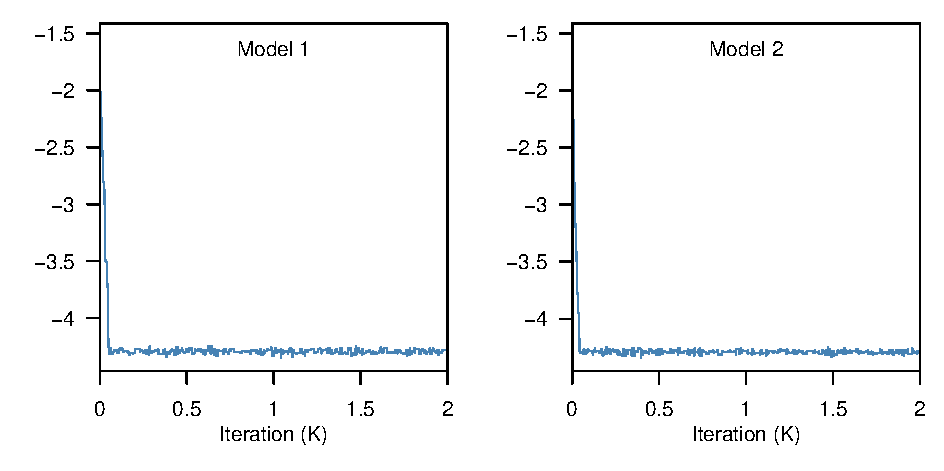
\includegraphics[width=\linewidth]{figures/03_NetworkModel/poc_traceplot_alpha.pdf}
    \caption{Trace plot of the baseline density parameter ($\alpha$) during the parameter recovery test. The chains, intentionally initialized at $\alpha=-2.0$, successfully demonstrate rapid convergence to the true parameter value ($\alpha \approx -4.29$) across both modeling frameworks.}
    \label{fig:poc_traceplot}
\end{figure}

\subsubsection{Adaptive MCMC Strategies}
To achieve practical computation times, simulations are conducted at a reduced scale of $N=1000$.
However, this reduction introduces a mathematical gap, or energy barrier, between the simulated statistics and the strict target distribution derived from the full dataset.
To overcome this barrier and ensure efficient parameter space exploration, we introduce an Adaptive MCMC framework.
This framework utilizes an Inflation factor to artificially widen the target covariance matrix during the initial stages.
Additionally, a Scaling factor is employed to dynamically adjust the proposal covariance matrix based on the empirical acceptance rate.

\paragraph{3.2.6.1 Model 1: Hybrid Two-Stage Scheduling}\mbox{}\\
The stochastic likelihood evaluation in Model 1 imposes a severe computational bottleneck if executed naively.
To optimize the trade-off between inference accuracy and computational cost, we designed a Two-Stage Adaptive MCMC architecture.
Phase 1 (Exploration) utilizes a computationally efficient single simulation ($n_{\text{sim}}=1$) alongside a gradually decreasing Inflation factor.
This phase rapidly explores the parameter space and learns an optimized proposal covariance matrix.
Phase 2 (Final Sampling) inherits this learned covariance matrix and executes the final sampling against the strict target (Inflation = 1).
By employing $n_{\text{sim}}=60$ simulations per step in this final phase, the stochastic noise is effectively smoothed without compromising the overall computational feasibility.

\begin{algorithm}[H]
\caption{Hybrid Two-Stage Adaptive MCMC for Model 1 (Stochastic Evaluation)}
\begin{algorithmic}[1]
\Require Initial parameters $\boldsymbol{\theta}_0$, Target statistics $\boldsymbol{\mu}_{\text{target}}, \boldsymbol{\Sigma}_{\text{target}}$
\Require Schedule of Inflation factors $\{I_1, I_2, \dots, I_S\}$ where $I_S = 1$
\Ensure Samples from the posterior distribution $p(\boldsymbol{\theta} \mid \text{Data})$

\Statex \textbf{Phase 1: Exploration with Adaptive Covariance ($n_{\text{sim}} = 1$)}
\State Initialize proposal covariance $\boldsymbol{\Sigma}_{\text{prop}}$
\For{stage $s = 1$ to $S-1$}
    \State Set current target covariance: $\boldsymbol{\Sigma}_{\text{stage}} = I_s \cdot \boldsymbol{\Sigma}_{\text{target}}$
    \For{iteration $i = 1$ to $M_{\text{stage}}$}
        \State Propose $\boldsymbol{\theta}^* \sim \mathcal{N}(\boldsymbol{\theta}_{i-1}, \boldsymbol{\Sigma}_{\text{prop}})$
        \State Generate a single network $\mathcal{G}^*$ given $\boldsymbol{\theta}^*$
        \State Compute summary statistics $S(\mathcal{G}^*)$
        \State Evaluate stochastic likelihood $\mathcal{L}(\boldsymbol{\theta}^*)$
        \State Accept/Reject $\boldsymbol{\theta}^*$ via Metropolis-Hastings ratio
    \EndFor
    \State Extract valid posterior samples $\boldsymbol{\Theta}_{\text{valid}}^{(s)}$ after burn-in
    \State Update $\boldsymbol{\Sigma}_{\text{prop}} \gets \mathrm{Cov}(\boldsymbol{\Theta}_{\text{valid}}^{(s)}) \cdot \text{ScalingFactor}$
\EndFor

\Statex \textbf{Phase 2: Final Sampling with LogSumExp Stabilization ($n_{\text{sim}} = 60$)}
\State Set target covariance strictly to $I_S = 1$: $\boldsymbol{\Sigma}_{\text{final}} = \boldsymbol{\Sigma}_{\text{target}}$
\For{iteration $i = 1$ to $M_{\text{final}}$}
    \State Propose $\boldsymbol{\theta}^* \sim \mathcal{N}(\boldsymbol{\theta}_{i-1}, \boldsymbol{\Sigma}_{\text{prop}})$
    \State Generate $n_{\text{sim}}=60$ independent networks $\mathcal{G}^*_1, \dots, \mathcal{G}^*_{60}$
    \State Compute log-likelihoods $LL_k$ for each $S(\mathcal{G}^*_k)$ against $\boldsymbol{\Sigma}_{\text{final}}$
    \State Approximate expected log-likelihood via LogSumExp: $\mathcal{L}_{\text{LSE}}(\boldsymbol{\theta}^*) = \max(LL) + \log \left( \frac{1}{60} \sum \exp(LL_k - \max(LL)) \right)$
    \State Accept/Reject $\boldsymbol{\theta}^*$ via Metropolis-Hastings ratio
\EndFor
\State \Return Final stationary chain from Phase 2
\end{algorithmic}
\end{algorithm}


\paragraph{3.2.6.2 Model 2: Unitary Adaptive Process}\mbox{}\\
As established in Section 3.2.5.2, the deterministic likelihood evaluation in Model 2 is free from simulation-induced noise.
Consequently, the chain stalling phenomenon observed in stochastic evaluation does not occur.
This renders the Two-Stage hybrid approach unnecessary for Model 2.
Instead, we employ a streamlined unitary adaptive process utilizing a standard covariance updating scheme.
This deterministic algorithm efficiently traverses the high-dimensional parameter space and achieves rapid convergence.

\begin{algorithm}[H]
\caption{Adaptive MCMC for Model 2 (Deterministic Evaluation)}
\begin{algorithmic}[1]
\Require Initial parameters $\boldsymbol{\theta}_0$, Target statistics $\boldsymbol{\mu}_{\text{target}}, \boldsymbol{\Sigma}_{\text{target}}$
\Require Pre-sampled CRN matrix $\mathbf{U}$ for latent variables $Z_i \sim \mathcal{N}(0,1)$
\Require Schedule of Inflation factors $\{I_1, I_2, \dots, I_S\}$ where $I_S = 1$
\Ensure Samples from the posterior distribution $p(\boldsymbol{\theta} \mid \text{Data})$

\State Initialize proposal covariance $\boldsymbol{\Sigma}_{\text{prop}}$
\For{stage $s = 1$ to $S$}
    \State Set current target covariance: $\boldsymbol{\Sigma}_{\text{stage}} = I_s \cdot \boldsymbol{\Sigma}_{\text{target}}$
    \For{iteration $i = 1$ to $M_{\text{stage}}$}
        \State Propose $\boldsymbol{\theta}^* \sim \mathcal{N}(\boldsymbol{\theta}_{i-1}, \boldsymbol{\Sigma}_{\text{prop}})$
        \State Analytically compute expected network statistics via LLN given $\mathbf{U}$ and $\boldsymbol{\theta}^*$
        \State Evaluate deterministic likelihood $\mathcal{L}(\boldsymbol{\theta}^*)$
        \State Accept/Reject $\boldsymbol{\theta}^*$ via Metropolis-Hastings ratio
    \EndFor
    \State Extract valid posterior samples $\boldsymbol{\Theta}_{\text{valid}}^{(s)}$ after burn-in
    \State Update $\boldsymbol{\Sigma}_{\text{prop}} \gets \mathrm{Cov}(\boldsymbol{\Theta}_{\text{valid}}^{(s)}) \cdot \text{ScalingFactor}$
\EndFor
\State \Return Final stationary chain from stage $S$
\end{algorithmic}
\end{algorithm}


\subsubsection{MCMC Diagnostics (Convergence Check)}
To validate the soundness of the proposed inference engine, the stationarity and convergence of the MCMC chains were rigorously assessed using both visual and quantitative diagnostics.
Visual inspection was conducted using trace plots to confirm optimal, caterpillar-like mixing across the parameter space.
Quantitatively, convergence across multiple independent chains was evaluated using the Gelman-Rubin potential scale reduction factor ($\hat{R}$).
A threshold of $\hat{R} < 1.1$ was established to mathematically ensure that all chains successfully converged to the same stationary posterior distribution.
Furthermore, the Effective Sample Size (ESS) was calculated for each parameter to verify that a sufficient number of independent samples were drawn, minimizing the impact of autocorrelation.
Across all final inference runs for Model 1, Model 2A, and Model 2B, every parameter successfully achieved $\hat{R} \le 1.02$.
Additionally, the ESS values substantially exceeded standard minimum thresholds, ranging from approximately 800 to over 2000, thereby guaranteeing highly robust and reliable posterior estimates.

\paragraph{3.2.7.1 Diagnostics for Model 1: Overcoming Stochasticity}\mbox{}\\
Figure \ref{fig:model1_comparison} illustrates the trace plot transition for the baseline density parameter ($\alpha$) during the Model 1's Phase 1 inference.
As intended by the hybrid architectural design, Phase 1 facilitated broad parameter exploration while suppressing computational costs.
However, at the final stage of Phase 1 (Stage 6, Inflation = 1), the chain exhibits severe stagnation, where the trace plot becomes rigidly flat.
This failure occurs because, with $n_{\text{sim}}=1$, the stochastic noise of the likelihood estimator is too large relative to the strict target distribution, leading to a near-zero acceptance rate.
Upon transitioning to Phase 2 ($n_{\text{sim}}=60$, Inflation = 1), this stochastic noise was successfully smoothed using the LogSumExp stabilization.
This stabilization allowed the chain to immediately escape stagnation and sample consistently from the target posterior distribution.
This empirical evidence clearly demonstrates the critical necessity of the Two-Stage approach for stochastic network models.

\begin{figure}[H]
    \centering
    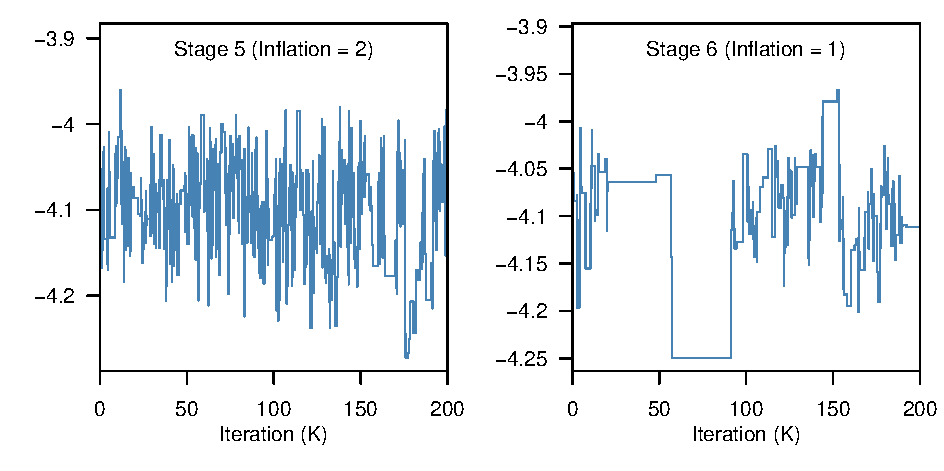
\includegraphics{figures/03_NetworkModel/model1_comparison_traceplot_alpha.pdf}
    \caption{Trace plot comparison for parameter $\alpha$ in Model 1, demonstrating the severe stagnation in Phase 1 (Stage 6: Inflation = 1, $n_{\text{sim}}=1$). The chain completely stalls due to stochastic noise exceeding the strict target tolerance.}
    \label{fig:model1_comparison}
\end{figure}

Figure \ref{fig:model1_stationary} presents the stationary trace plots for the four selected parameters ($\alpha$, $\phi_{ff}$, $\theta$, $\sigma_{re}$) throughout Phase 2.
The robust, caterpillar-like mixing observed across all four dimensions confirms that the $n_{\text{sim}}=60$ configuration provides sufficient likelihood stabilization.
Consequently, the MCMC algorithm successfully yielded a precise and fully converged posterior distribution for the stochastic baseline model.

\begin{figure}[H]
    \centering
    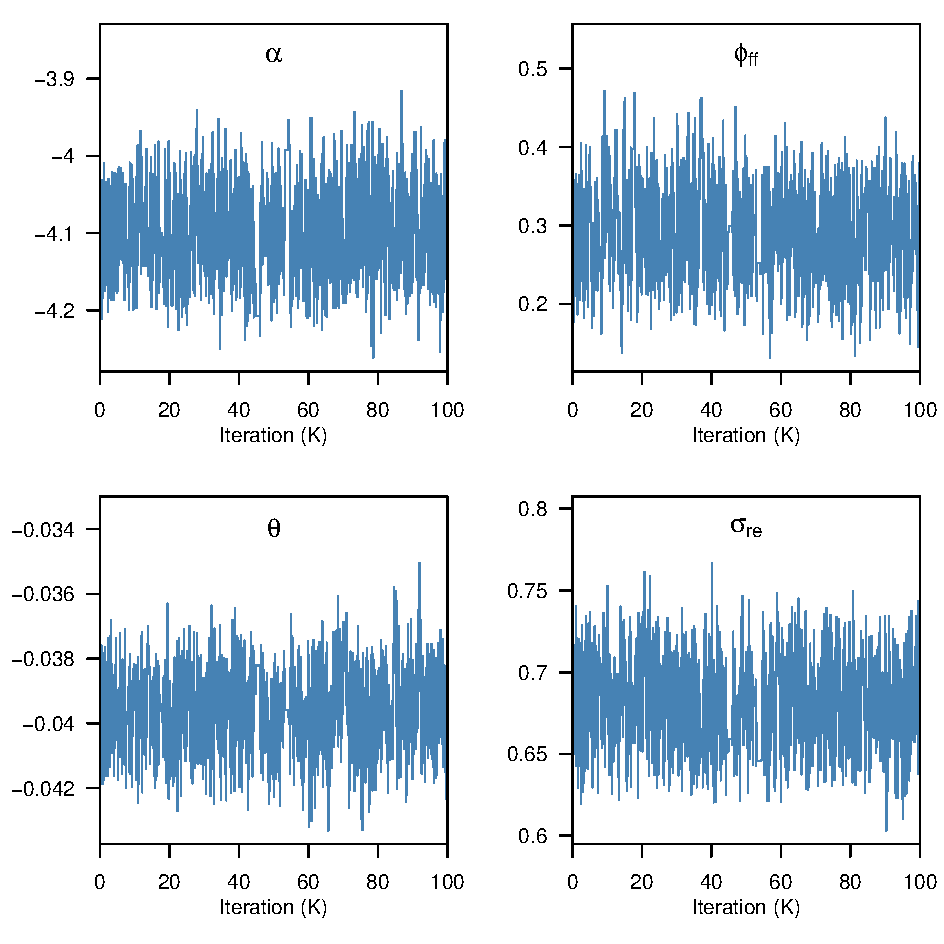
\includegraphics{figures/03_NetworkModel/model1_singlestage_traceplot.pdf}
    \caption{Stationary trace plots for the four primary parameters ($\alpha, \phi_{ff}, \theta, \sigma_{re}$) in Model 1 during Phase 2 ($n_{\text{sim}}=60$).
The consistent mixing across all dimensions indicates successful convergence to the posterior distribution.}
    \label{fig:model1_stationary}
\end{figure}


\paragraph{3.2.7.2 Diagnostics for Model 2: Deterministic Convergence}\mbox{}\\
For Model 2, the MCMC diagnostics confirm highly efficient and stable convergence due to the deterministic evaluation scheme.
Figure \ref{fig:model2_diagnostics} presents the trace plots for representative parameters of Model 2B.
These parameters capture key structural dimensions, including baseline density ($\alpha$), structural hierarchy ($\gamma_{\text{pri\_low}}$), attribute homophily ($\phi_{\text{mm}}$), and household generational heterogeneity ($\sigma_{\text{hhd}}$).
Unencumbered by probabilistic simulation noise, the parameter chains exhibit rapid mixing and establish a stationary distribution seamlessly within a single adaptive stage.
Comprehensive trace plots for all parameters across the variations are provided in the Appendix.

\begin{figure}[H]
    \centering
    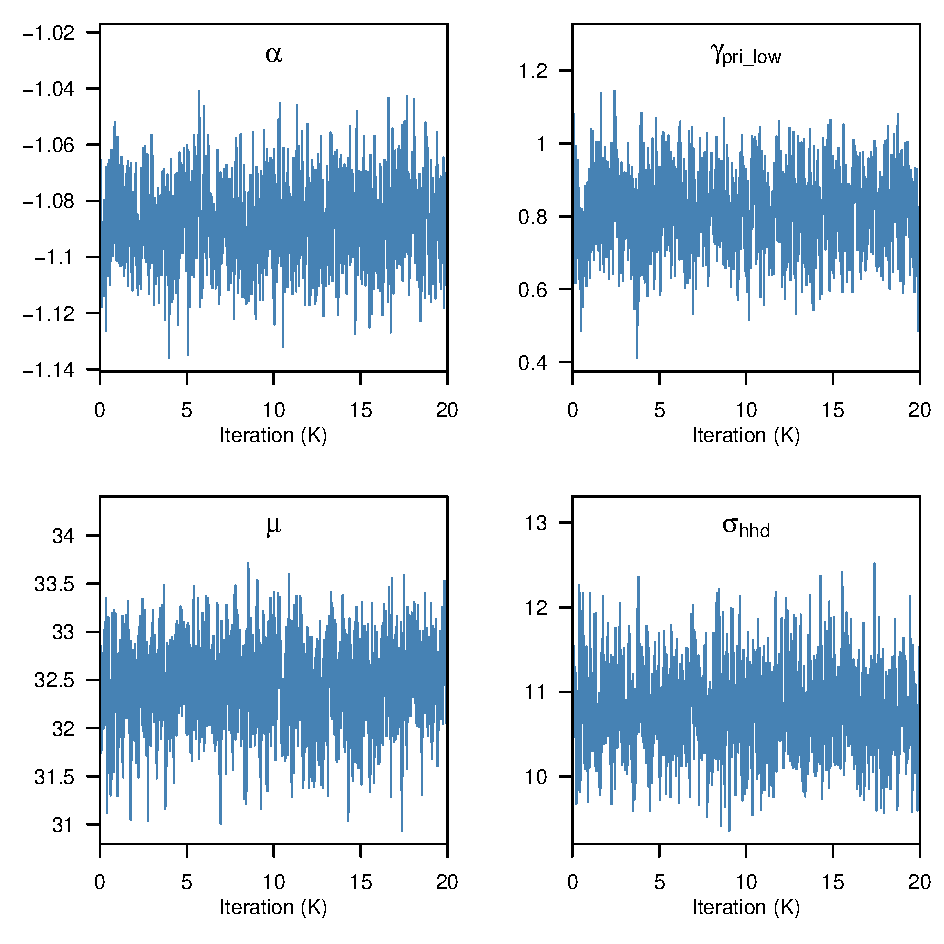
\includegraphics{figures/03_NetworkModel/model2b_singlestage_traceplot.pdf}
    \caption{MCMC diagnostic trace plots for representative parameters ($\alpha$, $\gamma_{\text{pri\_low}}$, $\phi_{\text{mm}}$, $\sigma_{\text{hhd}}$) in Model 2B, showing rapid and stable convergence.}
    \label{fig:model2_diagnostics}
\end{figure}
\subsection{Results}
\label{sec:results}

In this section, we systematically evaluate the generative performance of the proposed network models by comparing the simulated social contact patterns against the empirical POLYMOD dataset.
The assessment progresses from macroscopic network volume to microscopic, localized age-mixing structures, concluding with a holistic evaluation of the structural residuals.

\subsubsection{Summary Statistics Recovery and Structural Trade-offs}

Before examining the graphical properties of the generated networks, it is essential to verify the behavior of the Simulation-based Inference (SBI) engine.
Table \ref{tab:zscore_recovery} presents a comparison between the empirical target statistics and the posterior predictive distributions for Model 1 and Model 2B.
The accuracy of the parameter recovery is quantitatively assessed using Z-scores.
For Model 1, the highly flexible, generalized architecture allows the MCMC algorithm to perfectly calibrate to the macroscopic targets, resulting in Z-scores close to zero.
In contrast, Model 2B reveals a more nuanced, highly informative dynamic.
The strict, deterministic boundaries introduced to capture school cohorts successfully recovered their localized targets, with the proportions for Primary, Secondary, and Tertiary contacts all falling well within the acceptable $|Z| \le 2.0$ threshold.
However, this localized precision introduces a necessary bias-variance trade-off within the generative architecture.
By strictly constraining the model to reproduce rigid, step-like educational structures, the model sacrifices some degrees of freedom required to capture the extreme tails of the global degree distribution (e.g., the underestimation of super-spreaders, indicated by the large Z-score for $\text{Prop Degree} \ge 25$).
This discrepancy is not a failure of the inference, but rather a fundamental characteristic of highly stratified network models: enforcing strict local homophily inevitably restricts global distributional flexibility.
Having confirmed that the underlying structural rules were successfully extracted by the inference engine, the subsequent sections visually and quantitatively dissect how these localized rules manifest across the entire contact network.

\begin{table}[H]
    \centering
    \caption{Posterior predictive checks (Z-scores) for selected summary statistics. While Model 1 seamlessly fits broad macroscopic targets, Model 2B demonstrates a trade-off: it successfully captures rigid local structures (school cohorts) at the expense of extreme distributional tails.}
    \label{tab:zscore_recovery}
    \begin{tabular}{lccc}
        \toprule
        \textbf{Statistic} & \textbf{Empirical Target} & \textbf{Simulated Mean} & \textbf{Z-Score} \\
        \midrule
        \multicolumn{4}{l}{\textit{Panel A: Model 1 Targets}} \\
        Mean Degree & 13.53 & 13.67 & -0.13 \\
        Log Variance & 4.72 & 4.75 & -0.13 \\
        Mean Age Difference & 15.17 & 15.16 & 0.03 \\
        Proportion MM & 0.26 & 0.26 & 0.06 \\
        Proportion FF & 0.30 & 0.31 & -0.10 \\
        \midrule
        \multicolumn{4}{l}{\textit{Panel B: Model 2B Targets (Selected)}} \\
        Log Mean Degree & 2.61 & 2.59 & 1.90 \\
        Proportion Age 6--15 & 0.186 & 0.184 & 0.81 \\
        Proportion Primary Low & 0.028 & 0.025 & 1.65 \\
        Proportion Secondary & 0.097 & 0.102 & -1.46 \\
        Proportion Tertiary & 0.031 & 0.032 & -0.37 \\
        Proportion Degree $\ge 25$ & 0.148 & 0.123 & 11.26 \\
        \bottomrule
    \end{tabular}
\end{table}

\subsubsection{Macroscopic Network Volume and Degree Distribution}

The most fundamental characteristic of a contact network is its overall volume and the distribution of connections among individuals.
Figure \ref{fig:mean_degree} illustrates the mean total contacts across different age groups.
The empirical POLYMOD data reveals a distinct peak in contact volume among school-aged children and young adults, followed by a gradual decline in older populations.
Model 1, constrained by a uniform baseline density parameter, systematically underestimates the contact volume for younger cohorts and overestimates it for the elderly, resulting in a relatively flat degree profile.
In contrast, both Model 2A and Model 2B successfully reproduce the elevated contact rates among youths.
This improvement is directly driven by the integration of targeted educational attributes.

\begin{figure}[H]
    \centering
    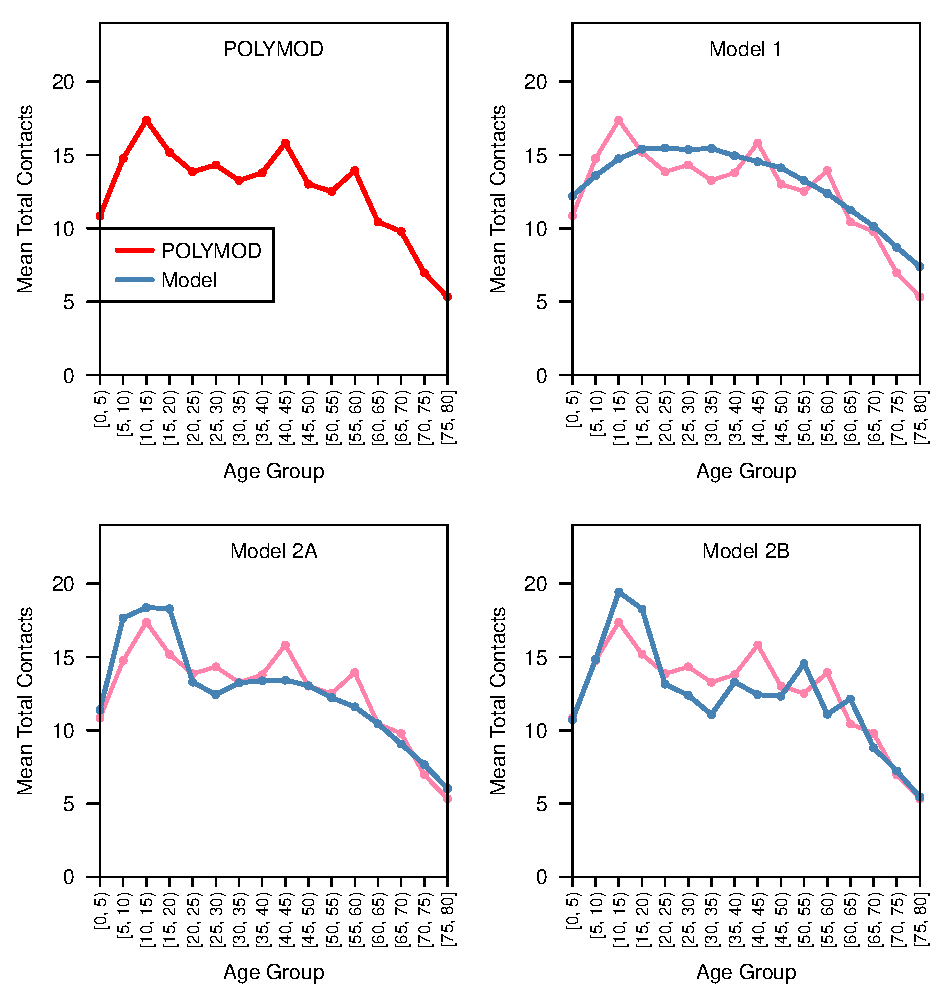
\includegraphics[width = 0.85\linewidth]{figures/03_NetworkModel/mean_degree_2x2.pdf}
    \caption{Comparison of mean total contacts (degree) by age group. Model 2 architectures successfully capture the elevated contact rates among younger populations compared to the flat profile of Model 1.}
    \label{fig:mean_degree}
\end{figure}

Beyond the mean values, examining the Cumulative Distribution Function (CDF) of the degree (Figure \ref{fig:degree_cdf}) provides critical insights into the dispersion of sociability.
Empirical contact networks are typically characterized by overdispersion, where a small fraction of highly sociable individuals acts as super-spreaders.
All three models effectively capture the broad shape of the empirical CDF.
This confirms that the individual-level random effect for sociability ($\epsilon_i$), introduced in the foundational equation, successfully models the variance and long-tail behavior of human interactions across all proposed architectures.

\begin{figure}[H]
    \centering
    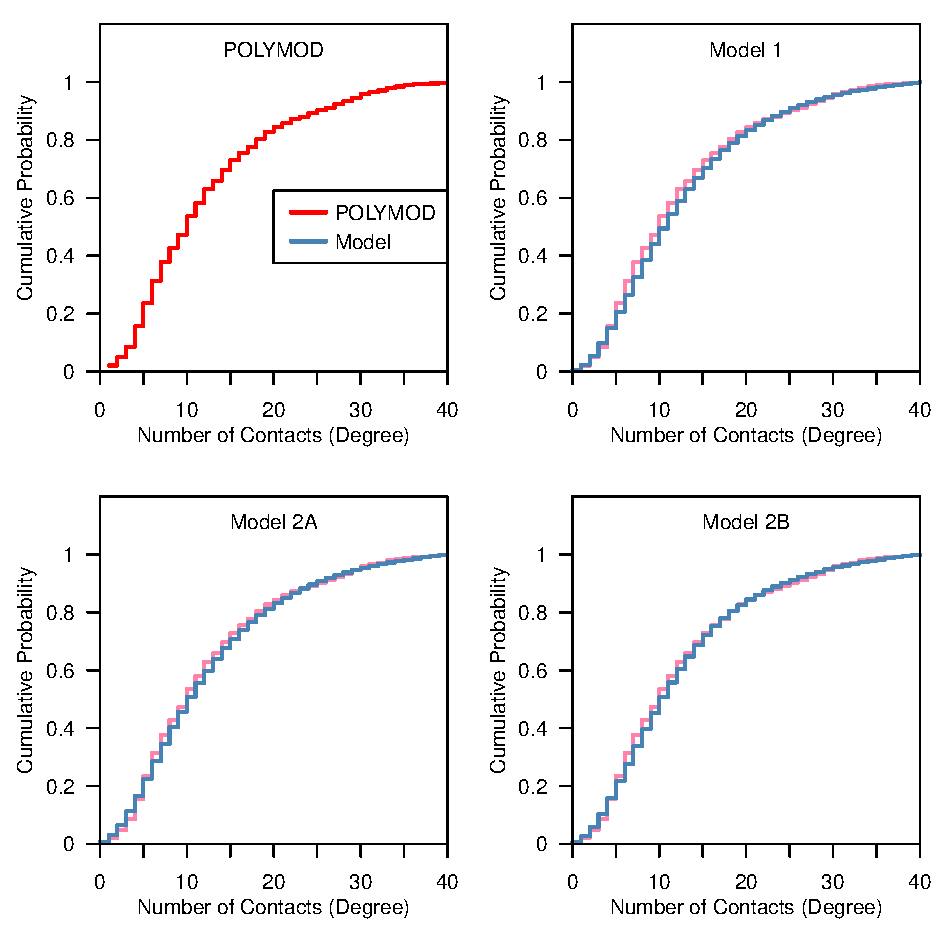
\includegraphics[width = 0.85\linewidth]{figures/03_NetworkModel/degree_cdf_2x2.pdf}
    \caption{Cumulative Distribution Function (CDF) of the number of contacts (degree). The node-specific random effects successfully capture the overdispersion and super-spreader tails across all models.}
    \label{fig:degree_cdf}
\end{figure}

\subsubsection{Meso-structure: Age Mixing Mechanisms}

While macroscopic metrics describe the overall volume of contacts, they do not capture the specific topological patterns of who interacts with whom.
Figure \ref{fig:agediff_dist} displays the probability distribution of absolute age differences between interacting individuals.
The empirical POLYMOD data exhibits a distinct bimodal characteristic: a sharp, exponentially decaying peak at an age difference of zero, representing intra-generational (peer) interactions, and a wider, normally distributed bump around 20 to 35 years, reflecting inter-generational (household) interactions.
Model 1 relies on a single continuous logit-linear function for age difference, resulting in a monotonically decreasing probability that completely fails to capture the inter-generational household bump.
By introducing a mixture distribution approach, both Model 2A and Model 2B successfully reproduce this complex bimodal mechanism.
They accurately generate both the sharp peer-to-peer spike and the broader parent-child mixing patterns.
This bimodal capture is further supported by the CDF of age differences shown in Figure \ref{fig:agediff_cdf}, where Model 2 architectures perfectly align with the empirical curve.

\begin{figure}[H]
    \centering
    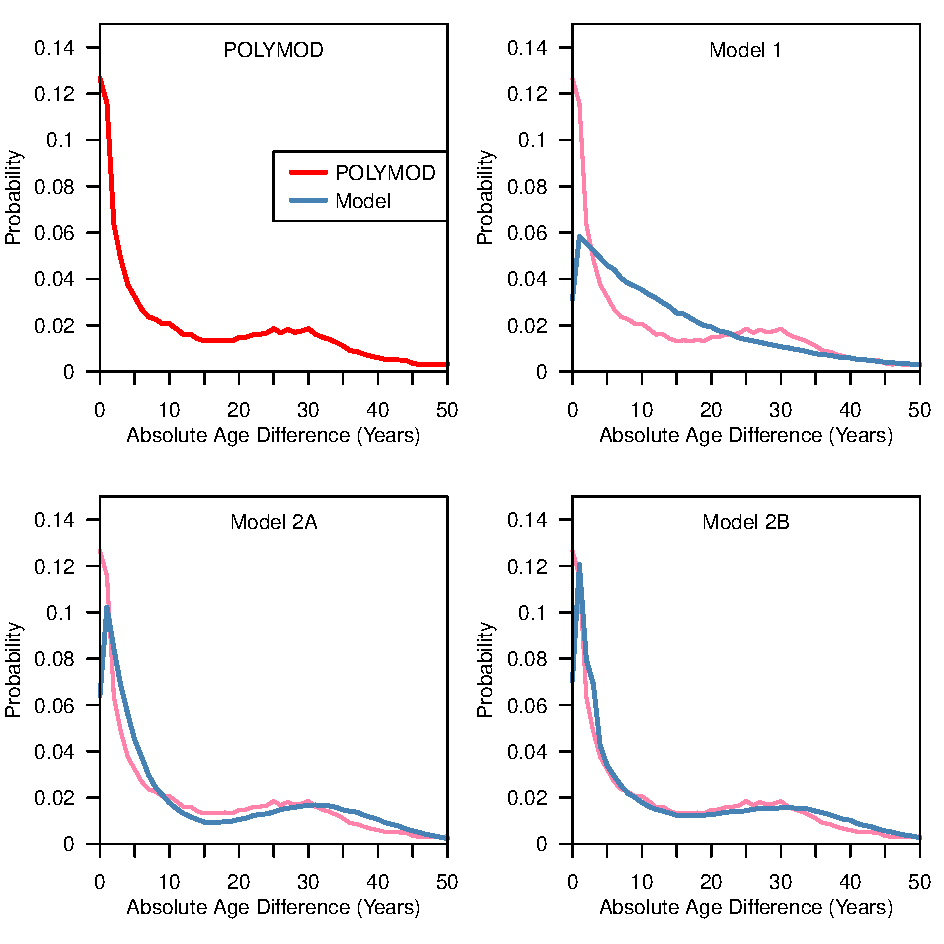
\includegraphics[width = 0.85\linewidth]{figures/03_NetworkModel/agediff_dist_2x2.pdf}
    \caption{Probability distribution of absolute age differences between contacting pairs. The mixture distribution in Model 2 successfully captures the bimodal nature of peer and household mixing.}
    \label{fig:agediff_dist}
\end{figure}

\begin{figure}[H]
    \centering
    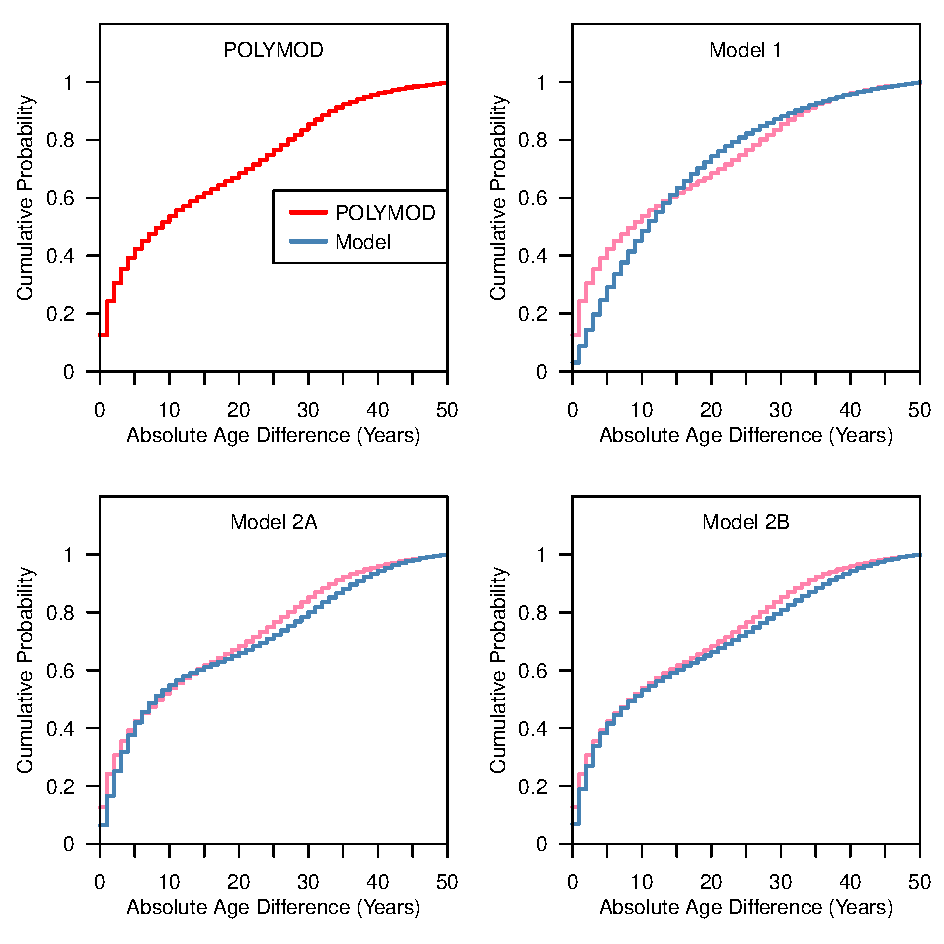
\includegraphics[width = 0.85\linewidth]{figures/03_NetworkModel/agediff_cdf_2x2.pdf}
    \caption{Cumulative Distribution Function (CDF) of absolute age differences, confirming the structural fit of the mixture distribution introduced in the Model 2 framework.}
    \label{fig:agediff_cdf}
\end{figure}

\subsubsection{Micro-structure: Localized Educational Homophily}

Although both Model 2A and 2B successfully capture macro-level and meso-level dynamics, their capabilities diverge significantly at the micro-structural level.
Figure \ref{fig:diag_step} isolates the diagonal elements of the contact matrix, representing the mean number of contacts occurring strictly within the same 5-year age cohort.
The empirical data displays a complex, step-like increase in peer contacts throughout childhood and adolescence, peaking dramatically in the $[10, 15)$ and $[15, 20)$ age groups before collapsing in adulthood.
Model 2A attempts to capture this phenomenon by applying a uniform educational homophily boundary across a broad $5 \le A \le 20$ range.
Consequently, Model 2A generates a flat, averaged plateau of peer contacts, failing to replicate the nuanced demographic gradients.
Conversely, Model 2B introduces highly localized, maximum-age-conditioned indicators representing Lower Primary, Upper Primary, Secondary, and Tertiary education.
This strict stratification allows Model 2B to perfectly fit the step-like empirical spikes.
This stark contrast clearly demonstrates that precise institutional boundaries are strictly required to accurately simulate micro-level societal interactions.

\begin{figure}[H]
    \centering
    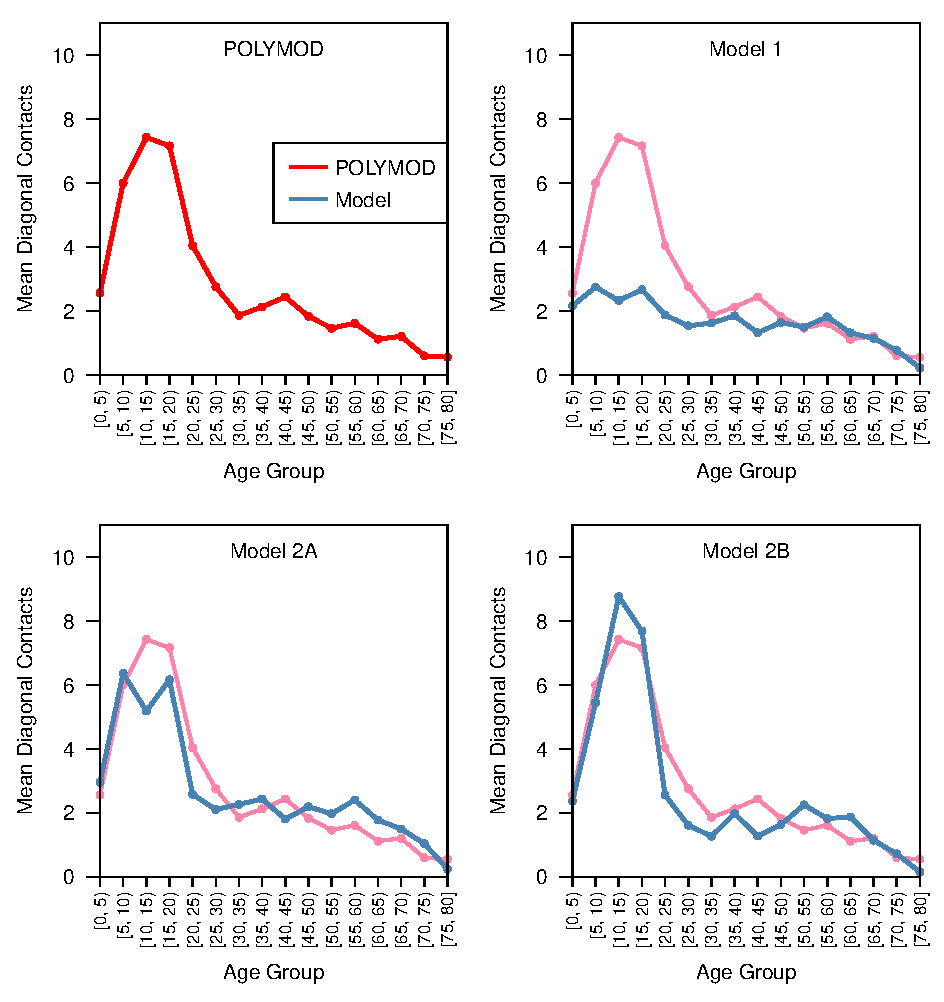
\includegraphics[width = 0.85\linewidth]{figures/03_NetworkModel/diag_step_2x2.pdf}
    \caption{Mean same-age-group (diagonal) contacts across 5-year age brackets. The strictly stratified boundaries in Model 2B are strictly necessary to capture the complex, step-like spikes in school-aged cohorts, exposing the limitations of the homogeneous approach in Model 2A.}
    \label{fig:diag_step}
\end{figure}

\subsubsection{Macro-Synthesis and Error Assessment}

To synthesize the localized micro-structural rules into a holistic perspective, we evaluate the full two-dimensional contact surface.
Figure \ref{fig:contact_matrix} visualizes the simulated contact matrices alongside the empirical POLYMOD matrix, while Figure \ref{fig:residual_matrix} explicitly plots the absolute residuals to highlight areas of systemic bias.
Model 1 exhibits severe, bright red structural residuals, particularly along the diagonal and the sub-diagonal bands, reflecting its inability to model concentrated school and household interactions.
Model 2B, by enforcing the intricate micro-rules discussed in previous sections, systematically neutralizes these systemic errors, resulting in a remarkably clean and white residual map.

\begin{figure}[H]
    \centering
    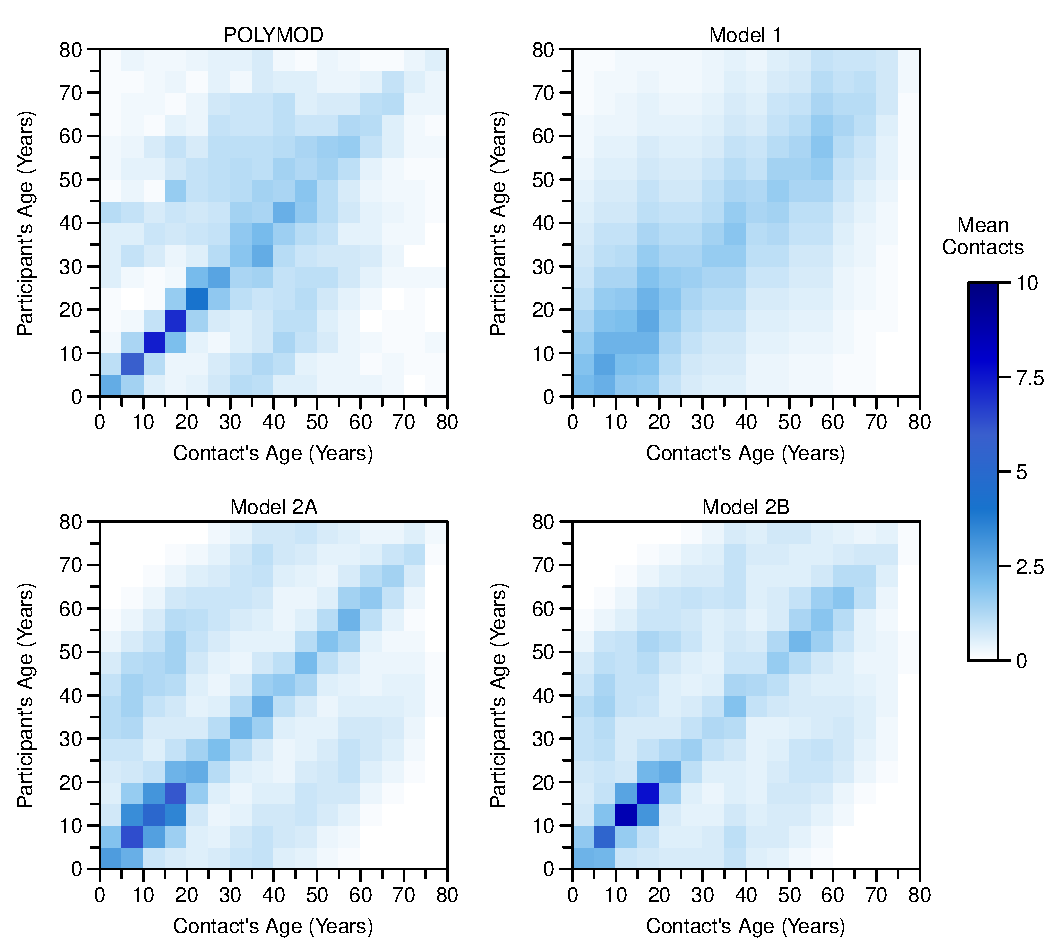
\includegraphics[width = \linewidth]{figures/03_NetworkModel/contact_matrix_2x2_legend.pdf}
    \caption{Two-dimensional contact matrices (heatmaps) comparing the generated networks against the empirical POLYMOD data.
    The intensity of the blue color represents the average number of contacts between individuals in the respective age groups, with more intense colors indicating a higher contact frequency.}
    \label{fig:contact_matrix}
\end{figure}

\begin{figure}[H]
    \centering
    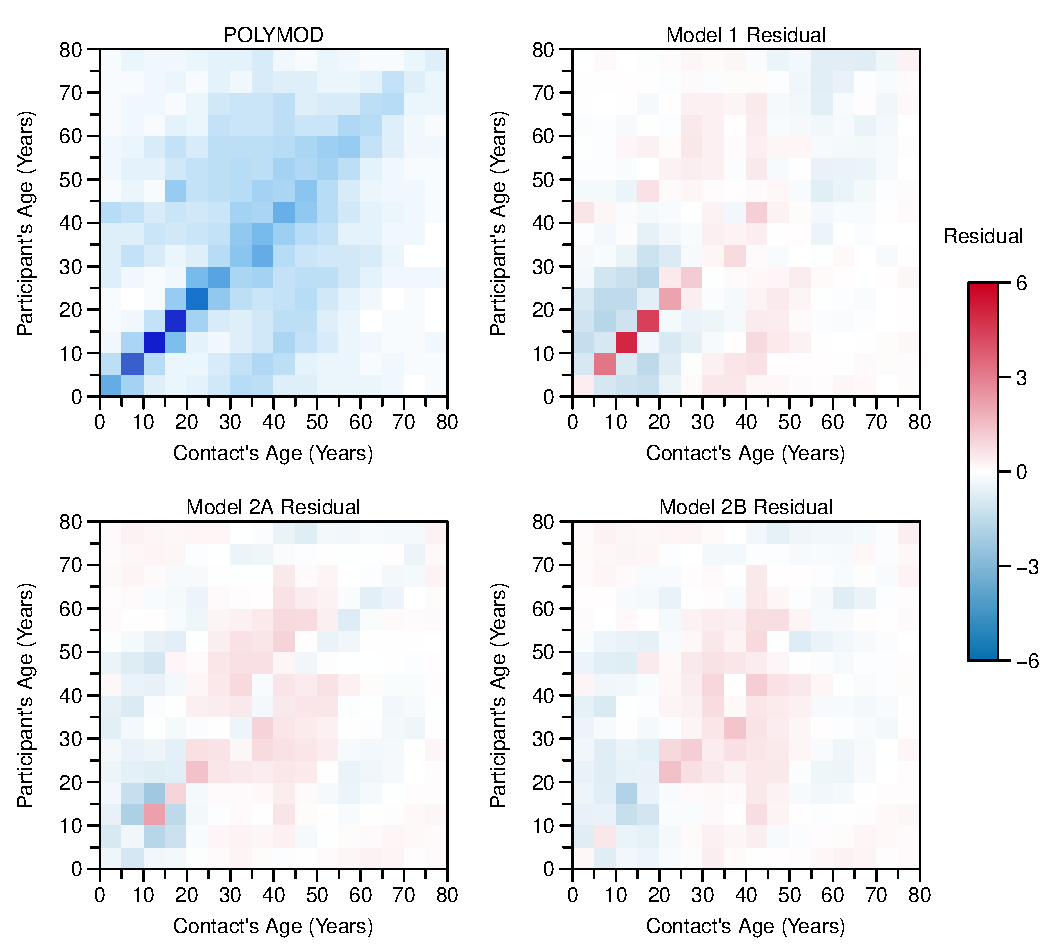
\includegraphics[width = \linewidth]{figures/03_NetworkModel/residual_matrix_2x2_legend.pdf}
    \caption{Heatmaps illustrating the model residuals.
    The panel in the top-left reproduces the empirical POLYMOD contact matrix for reference, identical to the one shown in Figure \ref{fig:contact_matrix}.
    The other three panels, titled 'model Residual,' display the difference between the empirical data and each model's predictions.
    A more intense red color indicates that the model underestimates the number of contacts for that specific age group cell, while a more intense blue color indicates an overestimation of contacts by the model.}
    \label{fig:residual_matrix}
\end{figure}

This visual synthesis is rigorously corroborated by the quantitative error metrics presented in Table \ref{tab:model_errors}.
The Mean Absolute Error (MAE) and Root Mean Squared Error (RMSE) were computed across three critical dimensions: the overall contact matrix, the mean degree, and the diagonal (same-age) contacts.
The data reveals a dramatic reduction in both Contact Matrix and Diagonal errors as the model complexity increases from Model 1 to Model 2B.
Notably, the Diagonal RMSE drops from 1.951 in Model 1 to 0.731 in Model 2B, mathematically validating the effectiveness of the strict educational stratification.
Interestingly, this extreme localized precision in Model 2B is accompanied by a slight increase in the Mean Degree error compared to Model 2A.
As foreshadowed by the Z-score analysis, this is a textbook manifestation of the bias-variance trade-off.
By sacrificing a marginal degree of global flexibility to satisfy rigid local constraints, Model 2B successfully achieves its primary objective: reconstructing the highly specific, localized transmission pathways that are essential for accurate epidemic modeling.

\begin{table}[H]
    \centering
    \caption{Quantitative error metrics (MAE and RMSE) for the three network models. The progression from Model 1 to Model 2B demonstrates a massive reduction in structural residuals (Contact Matrix and Diagonal), offset by a slight, necessary trade-off in the marginal mean degree.}
    \label{tab:model_errors}
    \begin{tabular}{lcccccc}
        \toprule
        & \multicolumn{2}{c}{Contact Matrix} & \multicolumn{2}{c}{Mean Degree} & \multicolumn{2}{c}{Diagonal Contacts} \\
        \cmidrule(lr){2-3} \cmidrule(lr){4-5} \cmidrule(lr){6-7}
        Model & MAE & RMSE & MAE & RMSE & MAE & RMSE \\
        \midrule
        Model 1  & 0.361 & 0.650 & 1.315 & 1.455 & 1.144 & 1.951 \\
        Model 2A & 0.334 & 0.480 & 1.102 & 1.505 & 0.637 & 0.817 \\
        Model 2B & 0.307 & 0.414 & 1.420 & 1.790 & 0.569 & 0.731 \\
        \bottomrule
    \end{tabular}
\end{table}

% 4. Epidemic Model
\section{Epidemic Model}
% 4_1_Model.tex
\subsection{Model}
\label{sec:epidemic_model}

To evaluate how network structures influence the spread of an infectious disease, we compare epidemic dynamics across four distinct contact networks, ordered by increasing structural resolution.
Each network is simulated with a fixed population size of $N = 10,000$ individuals.

\begin{enumerate}
    \item \textbf{Mean Field (MF) Model}:
    The Mean Field model serves as the homogeneous baseline for our stochastic simulations.
    It relies on the traditional assumption of perfect homogeneous mixing, where every individual has an equal probability of contacting any other individual in the population.
    Under this assumption, a single individual is effectively in contact with everyone else in the entire network.
    Consequently, this makes it the most unrealistic model among the four, entirely disregarding localized network structures and individual-level heterogeneity.

    \item \textbf{Erd\H{o}s-R\'enyi (ER) Model}:
    The Erd\H{o}s-R\'enyi model is a random graph where edges are formed with a uniform probability $p$.
    To ensure comparability, we calculated the probability $p$ such that the generated network matches the empirical mean degree ($\bar{k} \approx 13.5$) derived from the baseline POLYMOD data.
    The presence or absence of an edge between any two nodes is determined by an independent Bernoulli trial using this constant probability $p$.

    \item \textbf{Model 1 (Baseline Model)}:
    Model 1 represents a network generated without specific environmental contexts such as schools or households.
    It relies solely on basic age homophily and individual-level random effects for sociability.
    The existence of an edge between any pair of individuals is determined via an independent Bernoulli trial, utilizing the specific contact probability $P_{ij}$ derived from the logistic regression framework in Equation \ref{eq:m1_logit}.

    \item \textbf{Model 2 (Refined Model)}:
    Model 2 represents the most structurally realistic network in this study, corresponding to the fully stratified Model 2B.
    It incorporates strict age-bounded educational cohorts and intergenerational household mixing distributions.
    Similar to Model 1, the formation of each edge is simulated through an independent Bernoulli trial, based on the refined contact probability $P_{ij}$ defined in Equation \ref{eq:m2b_full}.
\end{enumerate}
% 4_2_Simulation.tex
\subsection{Simulation Conditions}
We implemented a stochastic Susceptible-Infected-Recovered (SIR) model using a discrete-time chain binomial process.
The population consists of $N = 10,000$ individuals, sampled based on the Year 2000 European demographic distribution.
The transition rules are defined as follows:

\textbf{Infection ($S \to I$):}
At each daily time step, a susceptible individual $i$ becomes infected with a probability dependent on the number of their currently infected neighbors, $I_{\text{neighbors}, i}$.
The probability of infection is given by:
$$P(S_i \to I_i) = 1 - \exp(-\rho \cdot I_{\text{neighbors}, i})$$
where $\rho$ is the per-contact transmission probability.
To ensure comparability across networks with different mean degrees $\bar{k}$, $\rho$ is analytically derived from the basic reproduction number $R_0$ using the relationship $\rho = -\log(1 - R_0 / \bar{k}) / d$.
In our primary scenario, we set $R_0 = 2.5$.
This value is selected to reflect the transmission potential observed in the early stages of the COVID-19 pandemic and other significant respiratory outbreaks \parencite{alimohamadi2020estimate, billah2020reproductive}.

\textbf{Recovery ($I \to R$):}
Infected individuals recover at a constant daily rate $\gamma$, independent of the network structure.
The duration of infection is set to $d = 7$ days, yielding a recovery probability of:
$$P(I \to R) = \gamma = \frac{1}{d}.$$

Each simulation is initialized with 5 infected individuals ($I_0 = 5$).
To reflect realistic outbreak origins, the initial nodes in the structured networks (Model 1 and 2) are selected with probabilities weighted by their degree, while random selection is used for the homogeneous models.
This degree-weighted initialization accounts for the higher probability of an outbreak being introduced or first detected among highly sociable "hubs" in the population \parencite{lloyd-smith2005superspreading}.
\subsection{Comparison of Epidemic Trajectories}
\label{sec:epidemic_comparison}

In this section, we analyze the macroscopic epidemic dynamics across the four proposed contact networks by performing 100 independent stochastic SIR simulations for each architecture.
Figure \ref{fig:sir_baseline} illustrates the resulting trajectories of susceptible, infected, and recovered populations, overlaid with the theoretical deterministic SIR curve calculated using Ordinary Differential Equations (ODEs).
As expected, the trajectories in the Mean Field (MF) and Erd\H{o}s-R\'enyi (ER) models closely align with the deterministic predictions, with average infection peaks of approximately 2,300 and 2,345 individuals, respectively.
The deterministic baseline provides a theoretical peak of 2,335 individuals occurring at Day 37.
Interestingly, the structured networks in Model 1 and Model 2 exhibit a significant departure from these homogeneous benchmarks.
In both Model 1 and Model 2, the infection peaks are notably higher and occur earlier than those predicted by the deterministic model and the ER network.
Specifically, the average stochastic peaks reached 2,634 individuals for Model 1 and 2,604 individuals for Model 2.
Furthermore, these structured models demonstrate a faster progression and an earlier termination of the outbreak compared to the MF and ER models.
While there are no substantial visual differences between the trajectories of Model 1 and Model 2 in this baseline scenario, both clearly highlight how demographic and institutional structures accelerate the initial phase of transmission.

\begin{figure}[H]
    \centering
    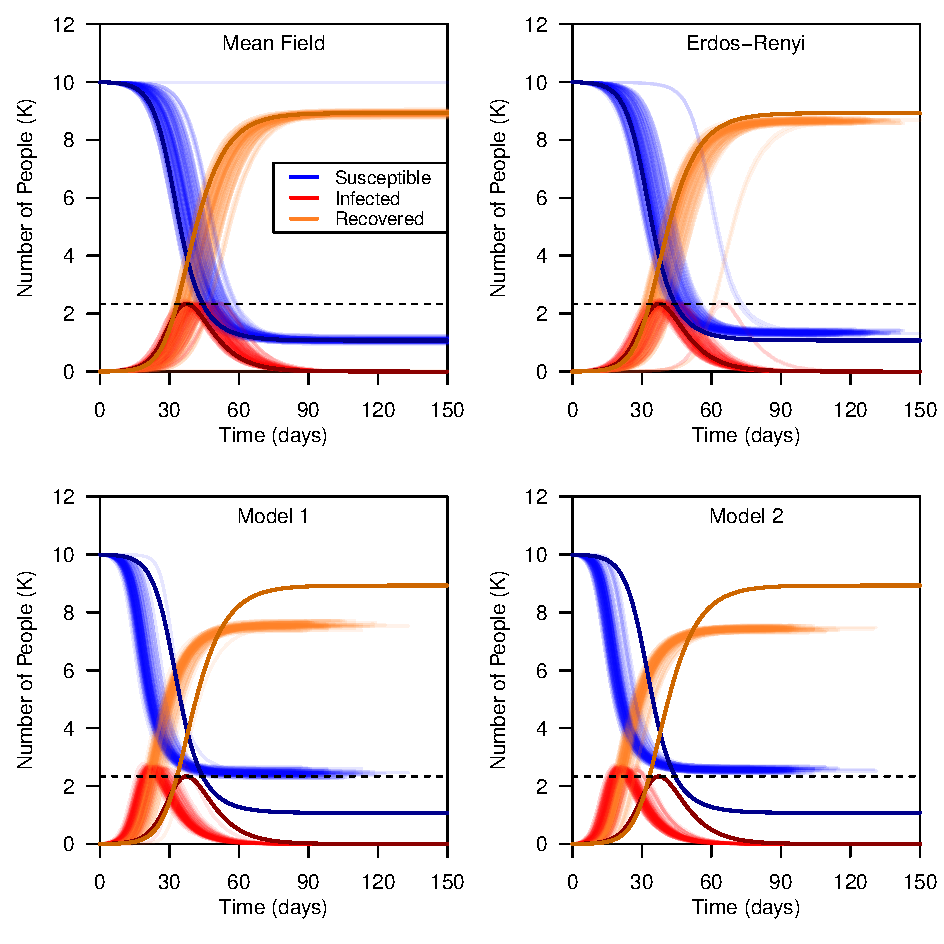
\includegraphics{figures/04_EpidemicModel/sir_baseline_r0_25.pdf}
    \caption{Stochastic SIR simulations across four baseline networks ($R_0 = 2.5$). The infection peaks in structured networks (Model 1 and Model 2) are higher and earlier than those in homogeneous models (Mean Field and Erd\H{o}s-R\'enyi) and the deterministic ODE prediction.}
    \label{fig:sir_baseline}
\end{figure}
\input{sections/04_EpidemicModel/4_4_DeepDive.tex}
% 4_5_SchoolIntervention.tex

\subsection{School Intervention}
This section evaluates the impact of targeted social distancing by simulating a school closure scenario across the four network models.
Rather than physically removing edges, the intervention is modeled as a probabilistic reduction by manipulating the underlying generative parameters.

\subsubsection{Definition and Target of Intervention}
In the structured Model 2B, the school intervention is defined by neutralizing the coefficients associated with educational settings.
Specifically, we modify Equation \ref{eq:m2b_full} by setting the parameters for school cohorts to zero: $\gamma_{pri\_low} = \gamma_{pri\_high} = \gamma_{sec} = \gamma_{ter} = 0$.
This allows us to calculate the intervention-adjusted contact probability, $P_{ij}^{close}$, for all pairs meeting the age-mixing criteria defined in Section \ref{sec:network_model}.
The baseline probabilities, $P_{ij}^{open}$, represent the state where schools are fully operational.

\subsubsection{Quantification of Reduction Factor}
To ensure a consistent magnitude of intervention across all models, we derived a standardized reduction factor, $R_{val}$.
This factor is calculated as the ratio of the total expected edges in the intervention scenario to those in the baseline scenario for the school-eligible population.
Let $\Omega$ be the set of individual pairs $(i, j)$ that satisfy the school cohort criteria.
The reduction factor is defined as:
\begin{equation}
    R_{val} = \frac{\sum_{(i,j) \in \Omega} P_{ij}^{close}}{\sum_{(i,j) \in \Omega} P_{ij}^{open}}.
\end{equation}
Based on our Model 2B posterior estimates, the calculated $R_{val}$ was approximately $0.2218$.
This indicates that a complete school closure corresponds to a reduction of approximately 77.8\% in the probability of contact between eligible youths within educational settings.

\subsubsection{Application to Baseline Models}
The reduction factor $R_{val}$ is subsequently applied to the Erd\H{o}s-R\'enyi and Model 1 networks to facilitate a fair comparison.
We identify "eligible" pairs in these models that satisfy the same age and age-difference boundaries as the school cohorts in Model 2B.
For these identified pairs, the baseline contact probability $P_{ij}^{M1, base}$ is scaled by the reduction factor:
\begin{equation}
    P_{ij}^{M1, interv} = P_{ij}^{M1, base} \times R_{val}.
\end{equation}
This methodology ensures that the total volume of contact reduction is identical across all models.
For the Erd\H{o}s-R\'enyi network, this reduction is operationalized by stochastically pruning edges of eligible pairs with probability $R_{val}$.
Crucially, during the subsequent SIR simulations, the per-contact transmission probability $\rho$ was kept constant at the baseline value.
This ensures that the pathogen's intrinsic infectiousness remains unaffected, allowing us to isolate the topological impact of the intervention.

\subsubsection{Comparative Analysis of Simulation Results}
Stochastic SIR simulations were performed to analyze the effectiveness of the intervention across different topologies, as visualized in Figure \ref{fig:sir_comparison}.
The results demonstrate that the effectiveness of school closure is highly sensitive to the underlying network structure.
In the Erd\H{o}s-R\'enyi model, the intervention yielded negligible changes in the epidemic trajectory, as the pathogen easily bypassed the localized reductions through the homogeneous background of contacts.
In Model 1, the average infection peak decreased from 2,634 to 2,545 individuals, representing a marginal reduction of only 3.37\%.
In contrast, Model 2B exhibited a significant suppression of the outbreak, with the peak incidence dropping from 2,604 to 2,282 individuals.
This substantial 12.3\% reduction in Model 2B is particularly noteworthy because it was achieved with the exact same volume of contact reduction as in Model 1.
The discrepancy highlights that in structured networks, school cohorts act as dense "transmission engines" or hubs.
Neutralizing these specific structural clusters breaks the core connectivity of the virus, leading to a non-linear suppression of the global peak.

\begin{figure}[H]
    \centering
    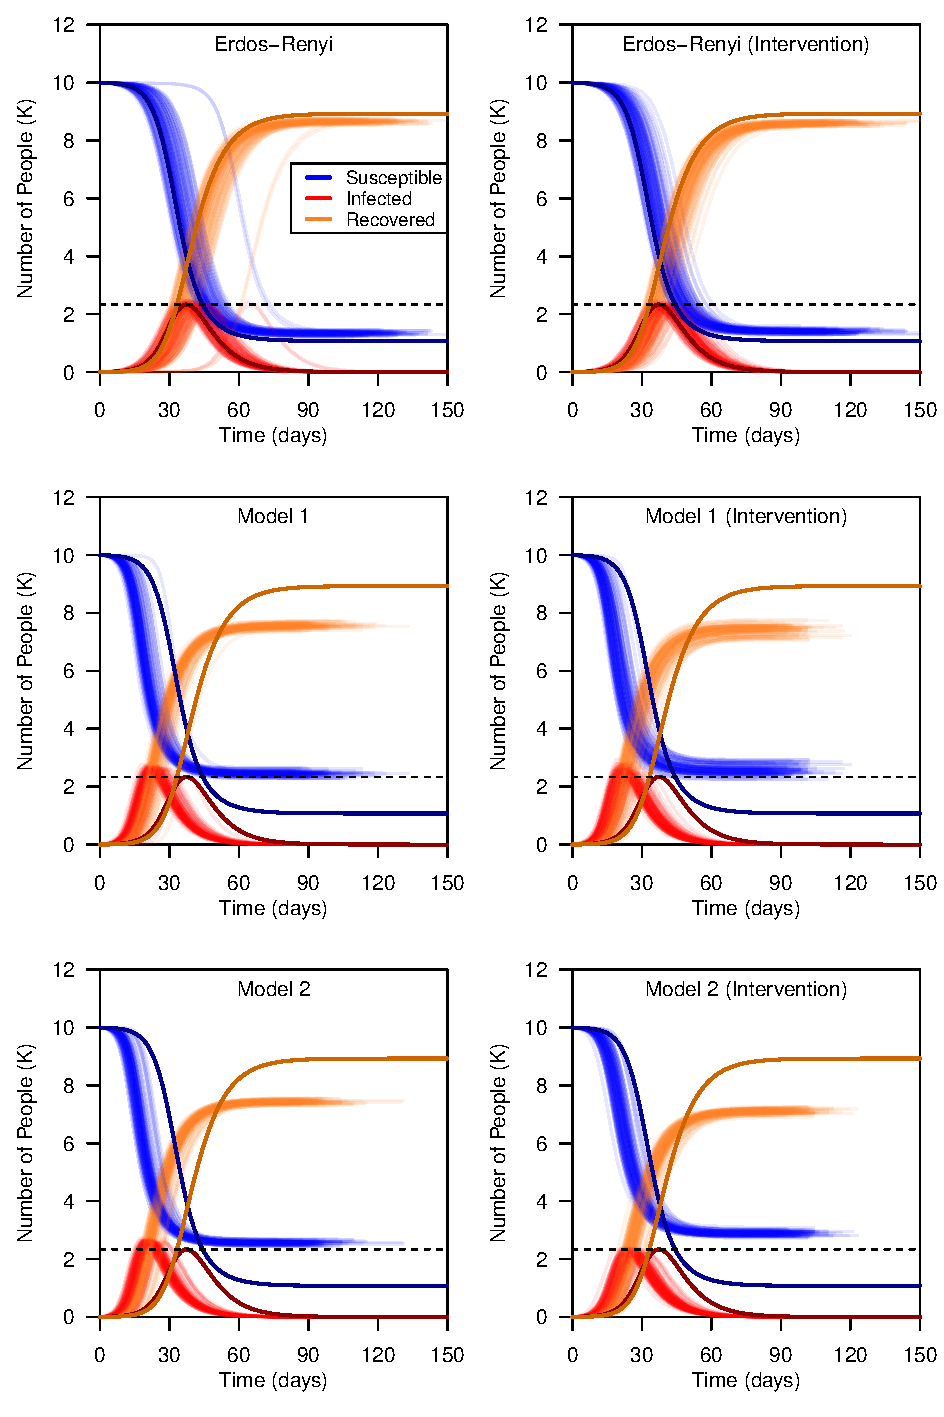
\includegraphics[width=0.8\linewidth]{figures/04_EpidemicModel/sir_comparison_r0_25.pdf}
    \caption{Comparison of SIR trajectories between Baseline and School Intervention scenarios ($R_0=2.5$). While the intervention has minimal impact on homogeneous models, it significantly suppresses the infection peak in Model 2B by dismantling dense school clusters.}
    \label{fig:sir_comparison}
\end{figure}

\subsubsection{Policy Implications and Limitations}
The findings of this study provide two critical insights for public health policy: the risk of overlooking epidemic acceleration and the potential for highly effective, targeted interventions.
First, the integration of realistic social layers reveals a significant risk of epidemic acceleration that is systematically overlooked in homogeneous models.
Our results demonstrate that when an outbreak occurs within structured environments like school cohorts, the pathogen exploits a high-speed "transmission highway" facilitated by dense local connectivity and high assortativity.
In these scenarios, the infection peak occurs both higher and significantly earlier than predicted by Mean Field or Erd\H{o}s-R\'enyi models.
Relying on oversimplified models for forecasting thus creates a dangerous "blind spot," where policymakers may systematically underestimate the urgency required for early-stage interventions.
Our model suggests that the window for effective peak suppression is much narrower than traditional models imply, making the timing of intervention as critical as its magnitude.

Second, the structural analysis identifies specific societal layers where interventions can yield disproportionately large impacts.
The 12.3\% reduction in the infection peak observed in Model 2B compared to only 3.37\% in Model 1 for the same volume of contact reduction proves that neutralizing "transmission engines" such as schools can non-linearly suppress the global outbreak.
This highlights the necessity of structured modeling to identify critical nodes and layers for precision public health strategies.

However, it is important to acknowledge that the potent suppression observed in Model 2B represents an optimistic scenario.
The model assumes that the edges removed through school closure are not replaced by other forms of interaction.
In reality, school closures may trigger "contact substitution," where students replace institutional interactions with informal social activities in the community.
Empirical evidence suggests that such behavioral shifts can significantly increase contacts within households and other private settings, potentially diminishing the intended impact of the closure \parencite{litvinova2019reactive}.
Such behavioral shifts could re-introduce random connectivity, potentially causing the network to revert toward a Model 1-like structure and diminishing the overall effectiveness of the policy.
Future research should incorporate these behavioral feedback loops to refine the predictability of layer-specific interventions and account for the dynamic nature of human sociality during a crisis.

% 5. Discussion
\section{Discussion}

\subsection{Key Insights}
The simulation results from the epidemic models highlight the critical role of network structure in the early phase of disease transmission.
Compared to homogeneous models such as the Erd\H{o}s-R\'enyi graph, our structured network (Model 2B), which explicitly incorporates educational cohorts and intergenerational mixing, demonstrated a substantially accelerated initial spread.
This acceleration is driven by highly connected "hubs" within the network, emphasizing that assuming homogeneous mixing underestimates the rapid onset of an outbreak.
Furthermore, our findings reveal the non-linear effects of targeted interventions.
An approach that uniformly reduces contact probabilities across the entire network (Model 1) resulted in a modest peak reduction of 3.37\%.
In contrast, targeting and disrupting specific cluster structures, such as school closures in Model 2B, yielded a disproportionately larger impact, achieving a 12.3\% reduction in the infection peak.
This demonstrates that interventions aimed at specific highly connected sub-populations are significantly more effective than broad, uniform contact reductions.

\subsection{Relationship to Existing Literature}
The importance of incorporating heterogeneity in social activity has been increasingly recognized in epidemiological modeling.
\textcite{britton2025improving} argue that accounting for the variation in the number of contacts within the same age group is essential for accurately predicting the basic reproduction number ($R_0$) and the final epidemic size.
Our Baseline Model (Model 1) directly addresses this by introducing a random effect for individual sociability, successfully capturing the dynamics where a subset of highly active individuals (potential super-spreaders) drives the initial transmission.
Moreover, while previous studies have underscored the significance of age homophily \parencite{mossong2008social} and location-specific micro-structures such as schools and workplaces \parencite{prem2017projecting}, constructing models that accurately reflect these features often requires complex demographic data.
Our approach successfully reconstructs these crucial structural properties using "age" as a single, versatile parameter, effectively bridging the gap between detailed contact surveys and practical network generation.

\subsection{Strengths and Limitations}
A major strength of this study lies in its computational statistical contributions.
Analytical likelihood calculation for infectious disease network models is notoriously difficult \parencite{mckinley2009inference}.
We overcame this challenge by employing a Synthetic Likelihood approach.
While high-dimensional inference often suffers from immense computational burden and the risk of getting trapped in local optima \parencite{ong2018likelihoodfree, picchini2023sequentially}, we engineered a robust inference pipeline.
The hybrid two-stage approach for Model 1 and the deterministic reparameterization for Model 2 ensured stable and efficient Markov Chain Monte Carlo (MCMC) convergence, providing a scalable solution for complex network inference.
However, the current study is not without limitations.
The most significant constraint is the static nature of the school closure simulations, which fail to capture behavioral feedback loops, specifically contact substitution.
Empirical evidence by \textcite{litvinova2019reactive} during reactive school closures in Russia showed that while contacts with classmates decreased significantly, contacts within the household increased by 40\% and with non-household relatives by 119\%.
Our current model does not account for this dynamic where lost contacts in one setting are compensated by increased interactions in another, potentially overestimating the effectiveness of the intervention.

\subsection{Remaining Gaps and Future Work}
Addressing the lack of contact substitution remains a priority for future research.
It is crucial to dynamically model behavioral shifts, such as the redistribution of surplus contact potential into the community and households when specific network layers (e.g., schools) are disrupted, as observed by \textcite{litvinova2019reactive}.
Additionally, in real-world epidemiological scenarios, complete network data is rarely available.
Future work should explore the extension of our inference framework to handle partially observed data.
Applying data augmentation techniques \parencite{bu2022likelihoodbased} or integrating compact mean-field models like the Edge-Based Compartmental Model (EBCM) with dynamic survival analysis \parencite{guzman2025inferring} could enable the reverse-engineering of underlying contact structures and the degree of behavioral substitution from limited epidemic outbreak data.

\subsection{Conclusion}
Homogeneous models that ignore the variance in individual sociability and structured cohorts severely underestimate the explosive acceleration of early-stage infections, leading to misguided predictions of intervention efficacy.
The integration of Synthetic Likelihood-based network inference with an epidemic model that explicitly represents social hubs provides a powerful and extensible foundation.
This framework paves the way for simulating more realistic public health interventions, ensuring that protocols like school closures can be evaluated accurately by anticipating risks such as contact substitution.

% References
\newpage
\printbibliography

\newpage
\section*{Change Log}
\addcontentsline{toc}{section}{Change Log}

\subsection*{1. Expansion and Clarification of Data Descriptions (Section 2)}
\begin{itemize}
    \item \textbf{Refinement of Prem et al. (2017) Description (Section 2.1):} Updated the methodology description regarding previous large-scale modeling efforts from "project and validate contact structures" to the more precise "construct and project synthetic contact matrices".
    \item \textbf{POLYMOD Data Utility (Section 2.1):} Clarified the conditions for the global applicability of the POLYMOD dataset. Added the nuance that "while macroscopic mixing patterns vary across countries", the setting-specific contact probabilities remain a gold standard for projecting transmission dynamics "when combined with local demographic data".
    \item \textbf{Specific Missing Value Ratios (Section 2.2):} Added the exact percentages of missing values in the data preprocessing section (approximately 0.12\% for contact age and 1.39\% for contact gender).
    \item \textbf{Wording Refinement (Section 2.3.1):} Removed the phrase "exhibits a realistic demographic profile" from the age distribution description for a more concise expression.
\end{itemize}

\subsection*{2. Enhancement of the Inference Engine Explanation (Section 3)}
\begin{itemize}
    \item \textbf{Removal of Unresolved Citation (Section 3.2.5.3):} Deleted the unresolved citation placeholder regarding the mean degree of the Erd\H{o}s-R\'{e}nyi graph.
    \item \textbf{Detailed Explanation of MCMC Stagnation (Section 3.2.7.1):} Fixed the MCMC diagnostics explanation for Model 1 to explicitly justify the algorithmic design of the Two-Stage approach.
    Added the exact failure mechanism in Phase 1: "with nsim = 1, the stochastic noise of the likelihood estimator is too large relative to the strict target distribution, leading to a near-zero acceptance rate" and severe stagnation where the trace plot becomes rigidly flat.
    Furthermore, explicitly stated that transitioning to Phase 2 utilizes "LogSumExp stabilization" to effectively smooth this noise, allowing the chain to immediately escape stagnation.
    \item \textbf{Figure 5 Caption Update:} Updated the caption for Figure 5 to reflect the newly added explanation, highlighting the "severe stagnation" and how the chain completely stalls due to stochastic noise exceeding the strict target tolerance.
\end{itemize}

\subsection*{3. Correction of Epidemic Model Definitions (Section 4)}
\begin{itemize}
    \item \textbf{Fixing Duplicated Baseline Models (Section 4.1):} Corrected an error in the baseline model list where "Model 1" was listed twice. The first model was properly replaced with the "Mean Field (MF) Model," and a description of its assumption of perfect homogeneous mixing was added.
\end{itemize}

\subsection*{4. Improvements in Figures, Formatting, and Typography}
\begin{itemize}
    \item \textbf{Addition of Legends to Matrix Heatmaps:} Added color bars (legends) to a total of three figures displaying contact and residual matrices (Figure 2, Figure 13, and Figure 14) to clearly indicate the numerical contact volume ("Mean Contacts") and error scale ("Residual") corresponding to each color intensity.
    \item \textbf{Proper Noun Correction:} Corrected the spelling of "Erdos-Renyi" to "Erd\H{o}s-R\'{e}nyi" with the proper accent marks throughout the document.
    \item \textbf{Typo Correction (Section 1):} Fixed the typo "highresolution" to "high resolution".
\end{itemize}

\subsection*{5. Major Additions to the Appendix}
Added a comprehensive Appendix section at the end of the final draft, which includes:
\begin{itemize}
    \item \textbf{Appendix A:} Density plots and QQ plots of the bootstrapped summary statistics to verify normality.
    \item \textbf{Appendix B:} Comprehensive MCMC trace plots for Model 1, Model 2A, and Model 2B.
    \item \textbf{Appendix C:} Detailed comparison tables of summary statistics (target mean, simulation mean, Z-score, and 95\% confidence intervals).
\end{itemize}

\subsection*{6. Change in Source Codes}
\begin{itemize}
    \item \texttt{src/assessment\_plot\_func.R:} Added a new function to generate the legend for the contact matrix heatmaps, which was missing in the original codebase.
    This function creates a color bar that maps the intensity of the blue color to the average number of contacts, allowing for clearer interpretation of the heatmaps in Figures 2, 13, and 14. 
    \item \texttt{Network\_22\_model\_assessment.qmd:} Updated the code to include the newly created legend function for the contact matrix heatmaps, ensuring that all relevant figures now contain the appropriate legends for better clarity and presentation.
\end{itemize}

\newpage
\appendix
\section*{Appendix: Bootstrap Distributions and Normality Checks}
\label{sec:appendix_bootstrap}

% ==========================================
% Model 1 (Base Model)
% ==========================================
\subsection*{A.1 Model 1}

\begin{figure}[htbp]
    \centering
    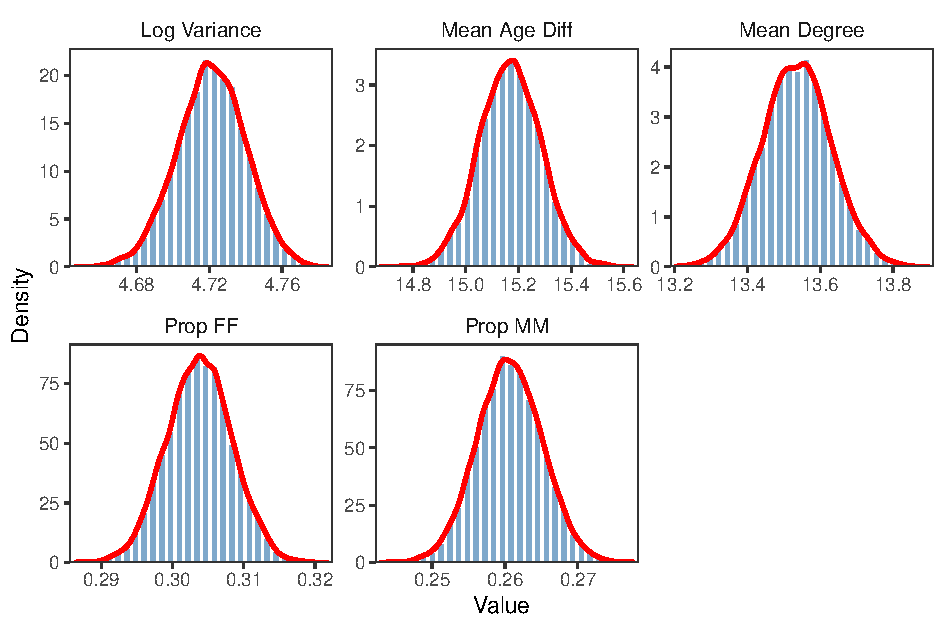
\includegraphics[width=0.9\textwidth]{figures/06_Appendix/density_bootstrap_m1.pdf}
    \caption{Density plots of the bootstrapped summary statistics for Model 1. The histograms represent the distribution of 10,000 bootstrap samples, overlaid with the estimated density curves (red lines).}
    \label{fig:density_m1}
\end{figure}

\begin{figure}[htbp]
    \centering
    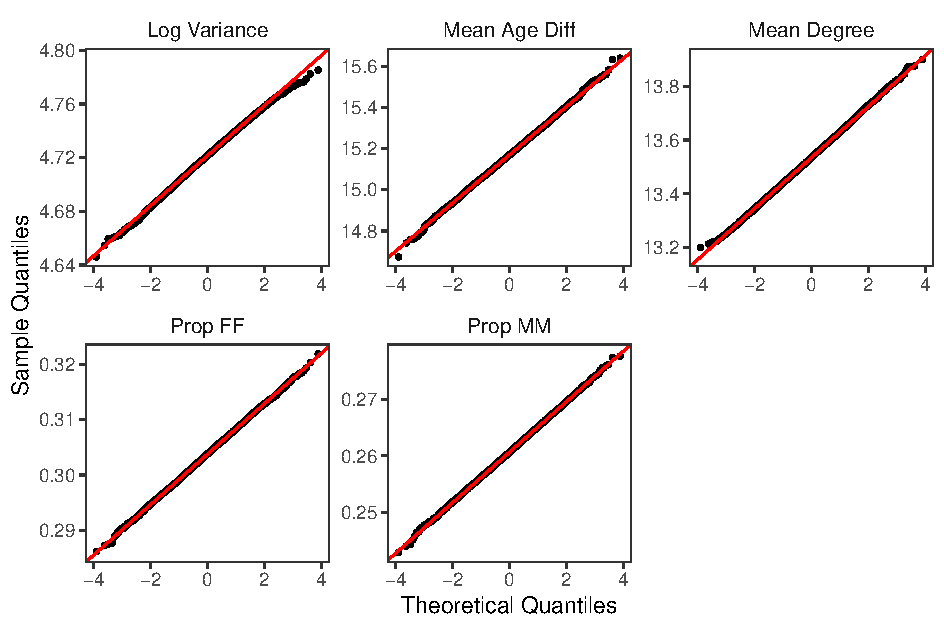
\includegraphics[width=0.9\textwidth]{figures/06_Appendix/qqplot_bootstrap_m1.pdf}
    \caption{QQ plots of the bootstrapped summary statistics for Model 1. The sample quantiles closely matching the theoretical normal quantiles (red lines) indicate that the statistics are approximately normally distributed.}
    \label{fig:qq_m1}
\end{figure}

\clearpage

% ==========================================
% Model 2A
% ==========================================
\subsection*{A.2 Model 2A}

\begin{figure}[htbp]
    \centering
    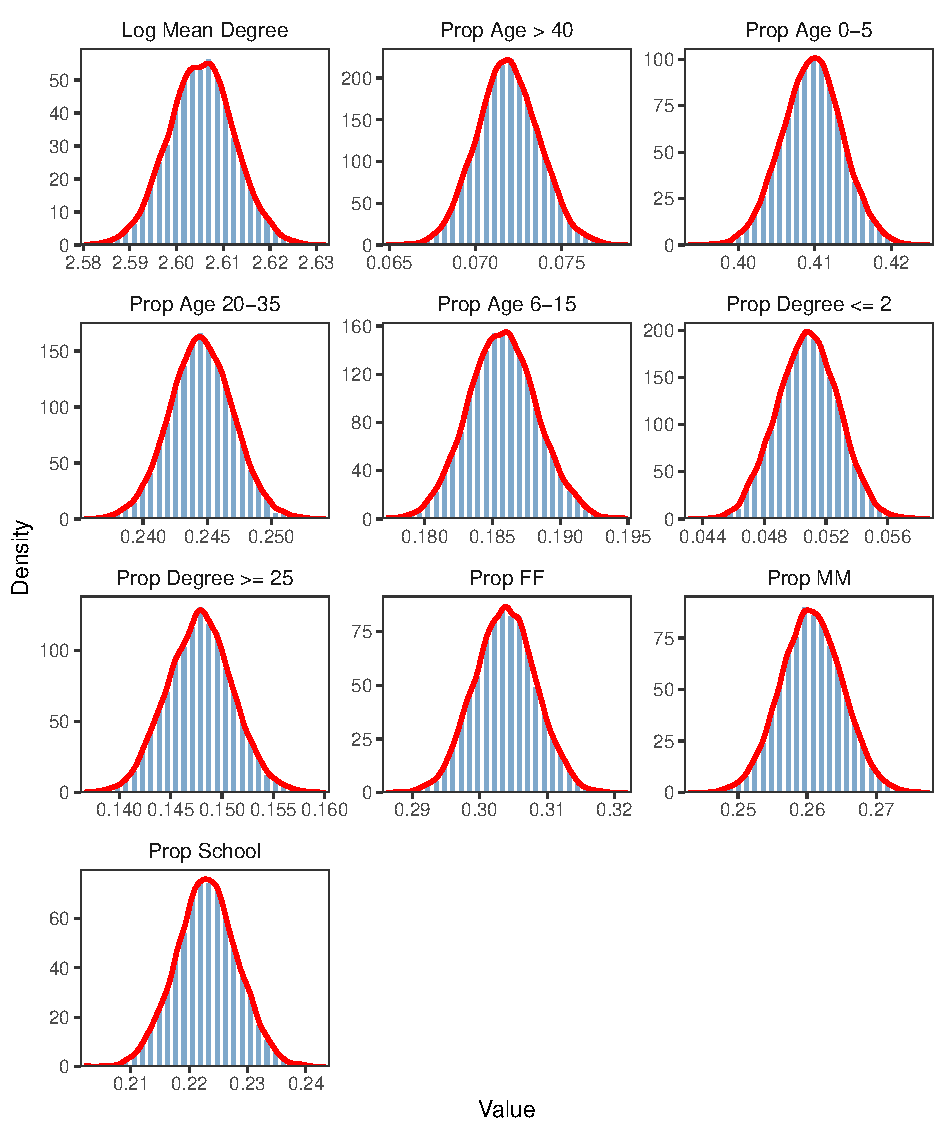
\includegraphics[width=0.85\textwidth]{figures/06_Appendix/density_bootstrap_m2a.pdf}
    \caption{Density plots of the bootstrapped summary statistics for Model 2A (10 variables).}
    \label{fig:density_m2a}
\end{figure}

\begin{figure}[htbp]
    \centering
    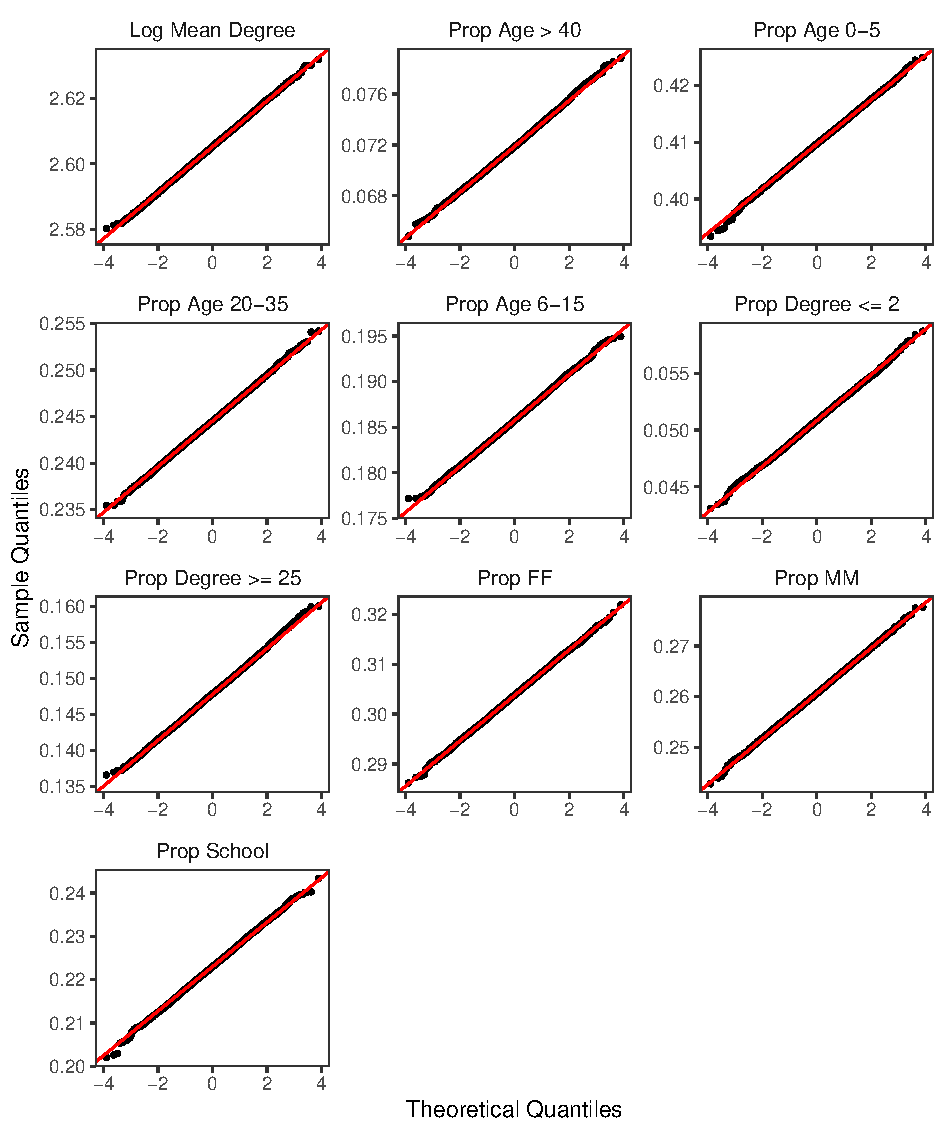
\includegraphics[width=0.85\textwidth]{figures/06_Appendix/qqplot_bootstrap_m2a.pdf}
    \caption{QQ plots of the bootstrapped summary statistics for Model 2A.}
    \label{fig:qq_m2a}
\end{figure}

\clearpage

% ==========================================
% Model 2B
% ==========================================
\subsection*{A.3 Model 2B}

\begin{figure}[htbp]
    \centering
    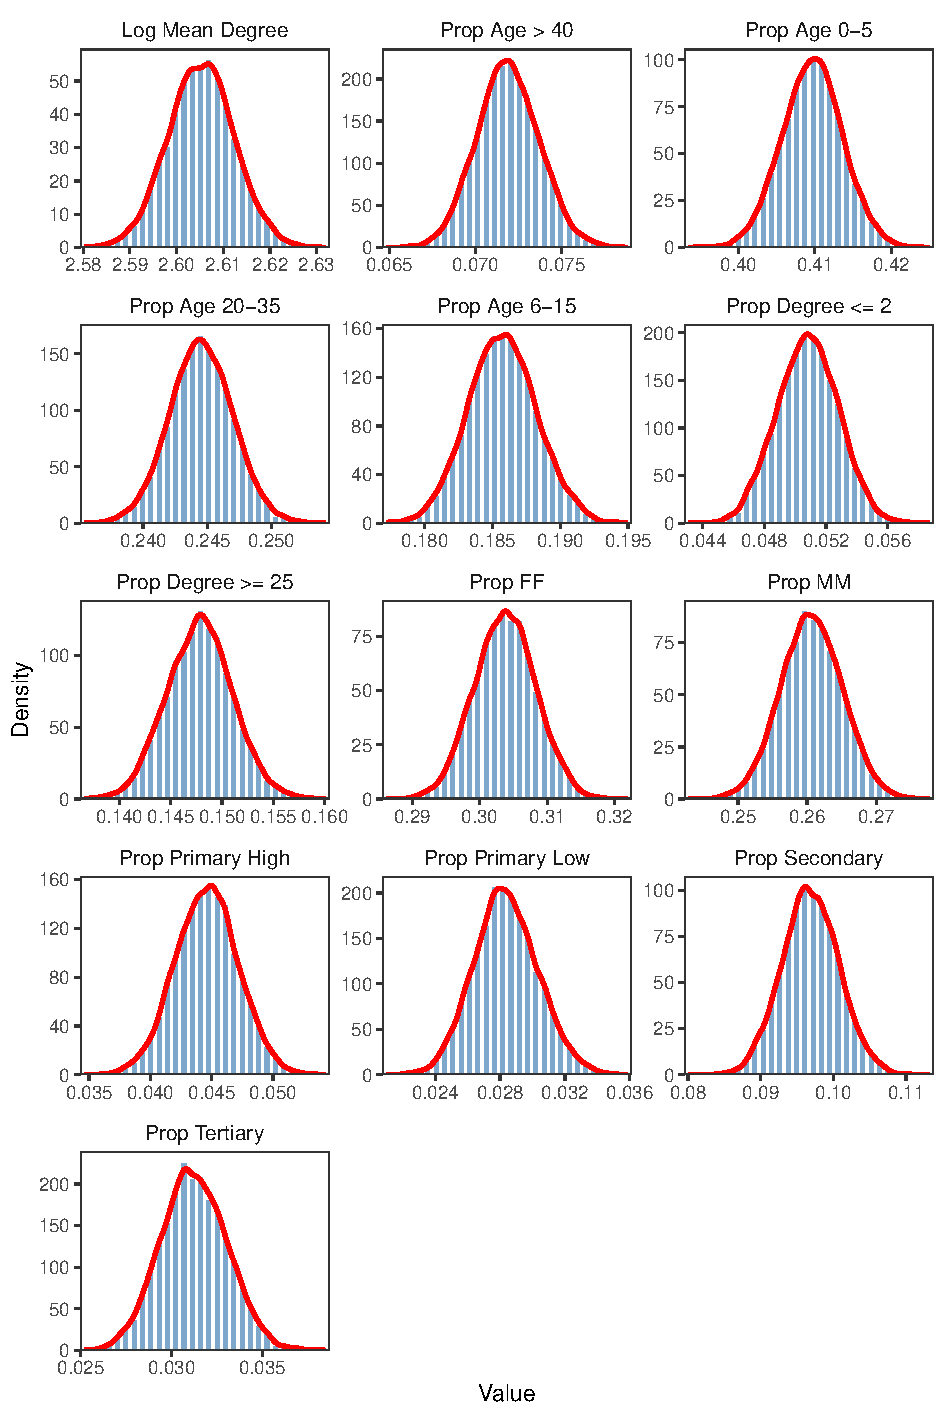
\includegraphics[width=0.7\linewidth]{figures/06_Appendix/density_bootstrap_m2b.pdf}
    \caption{Density plots of the bootstrapped summary statistics for Model 2B (13 variables).}
    \label{fig:density_m2b}
\end{figure}

\begin{figure}[htbp]
    \centering
    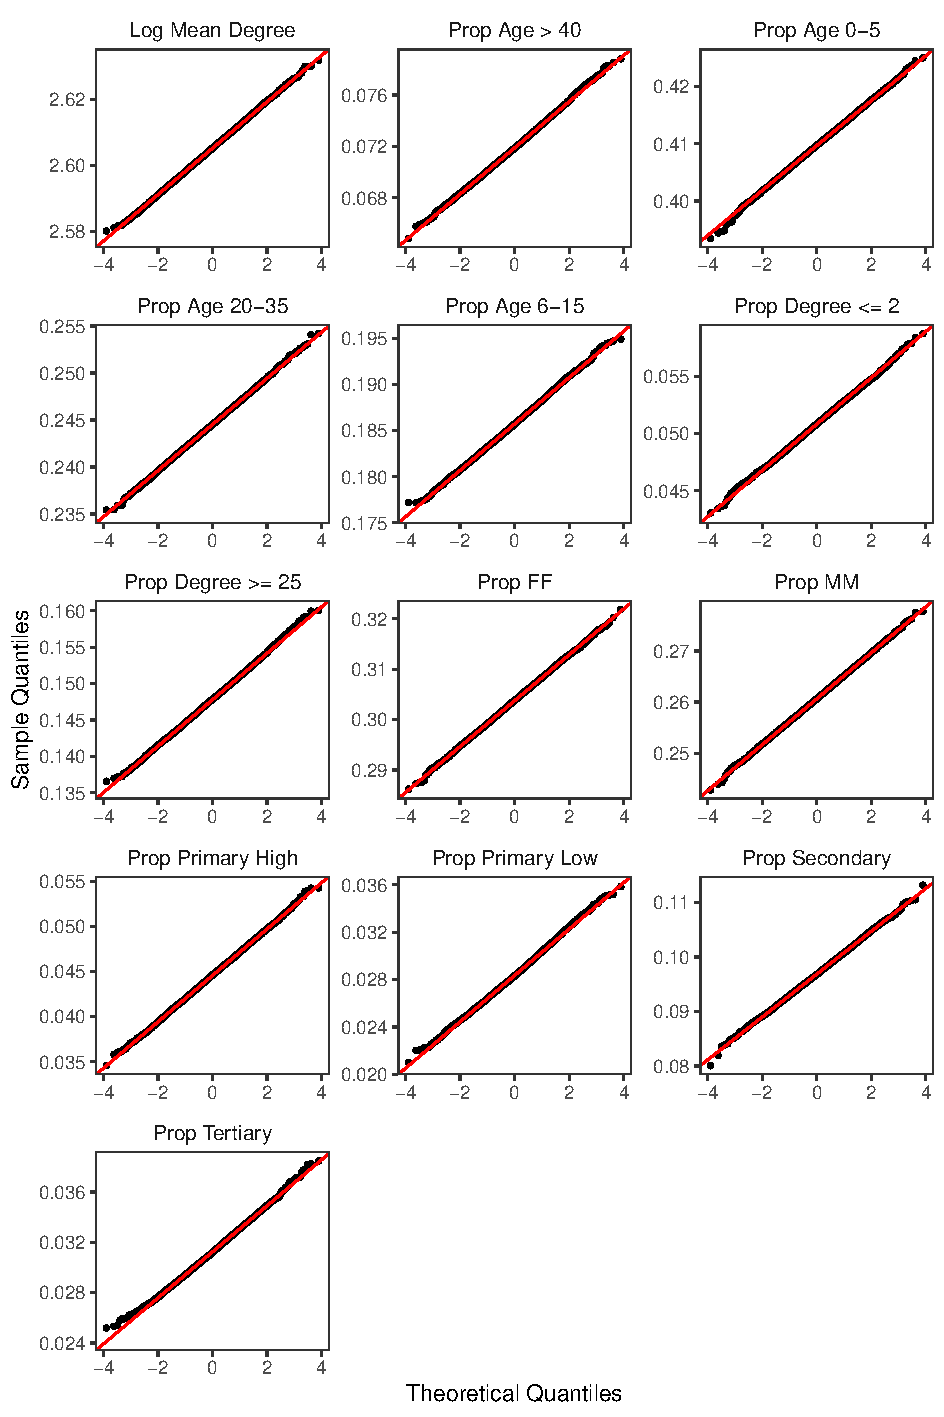
\includegraphics[width=0.7\textwidth]{figures/06_Appendix/qqplot_bootstrap_m2b.pdf}
    \caption{QQ plots of the bootstrapped summary statistics for Model 2B.}
    \label{fig:qq_m2b}
\end{figure}

\clearpage

\section*{Appendix: MCMC Trace Plots}
\label{sec:appendix_traceplots}

% ==========================================
% Model 1
% ==========================================
\subsection*{B.1 Model 1}

\begin{figure}[htbp]
    \centering
    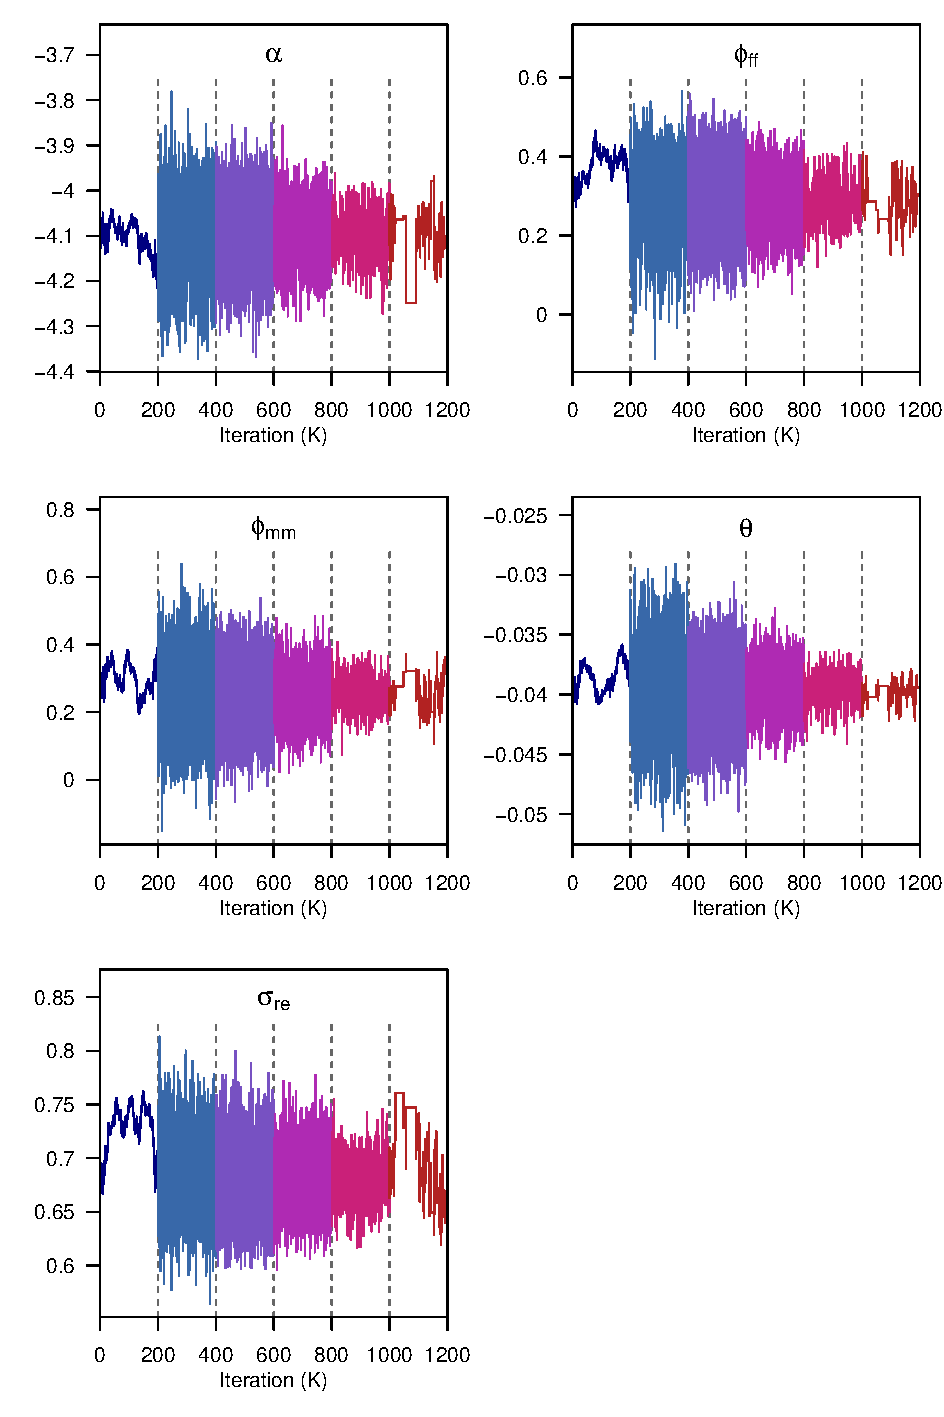
\includegraphics[width=0.75\textwidth]{figures/06_Appendix/model1_multistage_traceplot_1.pdf}
    \caption{Model 1: Multistage MCMC trace plots.}
    \label{fig:trace_m1_multi}
\end{figure}

\begin{figure}[htbp]
    \centering
    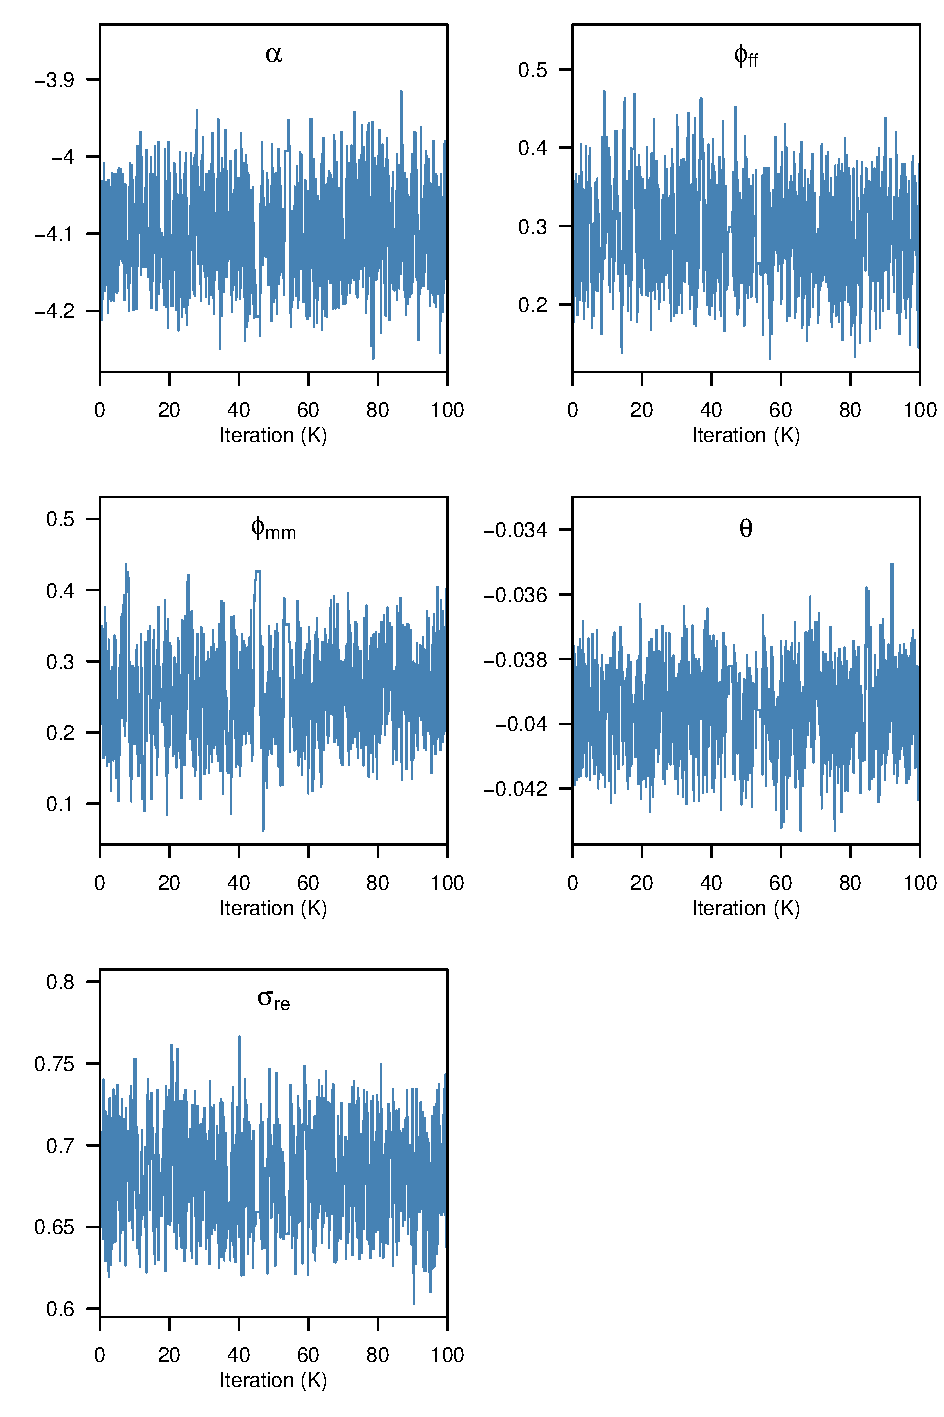
\includegraphics[width=0.85\textwidth]{figures/06_Appendix/model1_singlestage_traceplot_1.pdf}
    \caption{Model 1: Singlestage MCMC trace plots.}
    \label{fig:trace_m1_single}
\end{figure}

\clearpage

% ==========================================
% Model 2A
% ==========================================
\subsection*{B.2 Model 2A}

\begin{figure}[htbp]
    \centering
    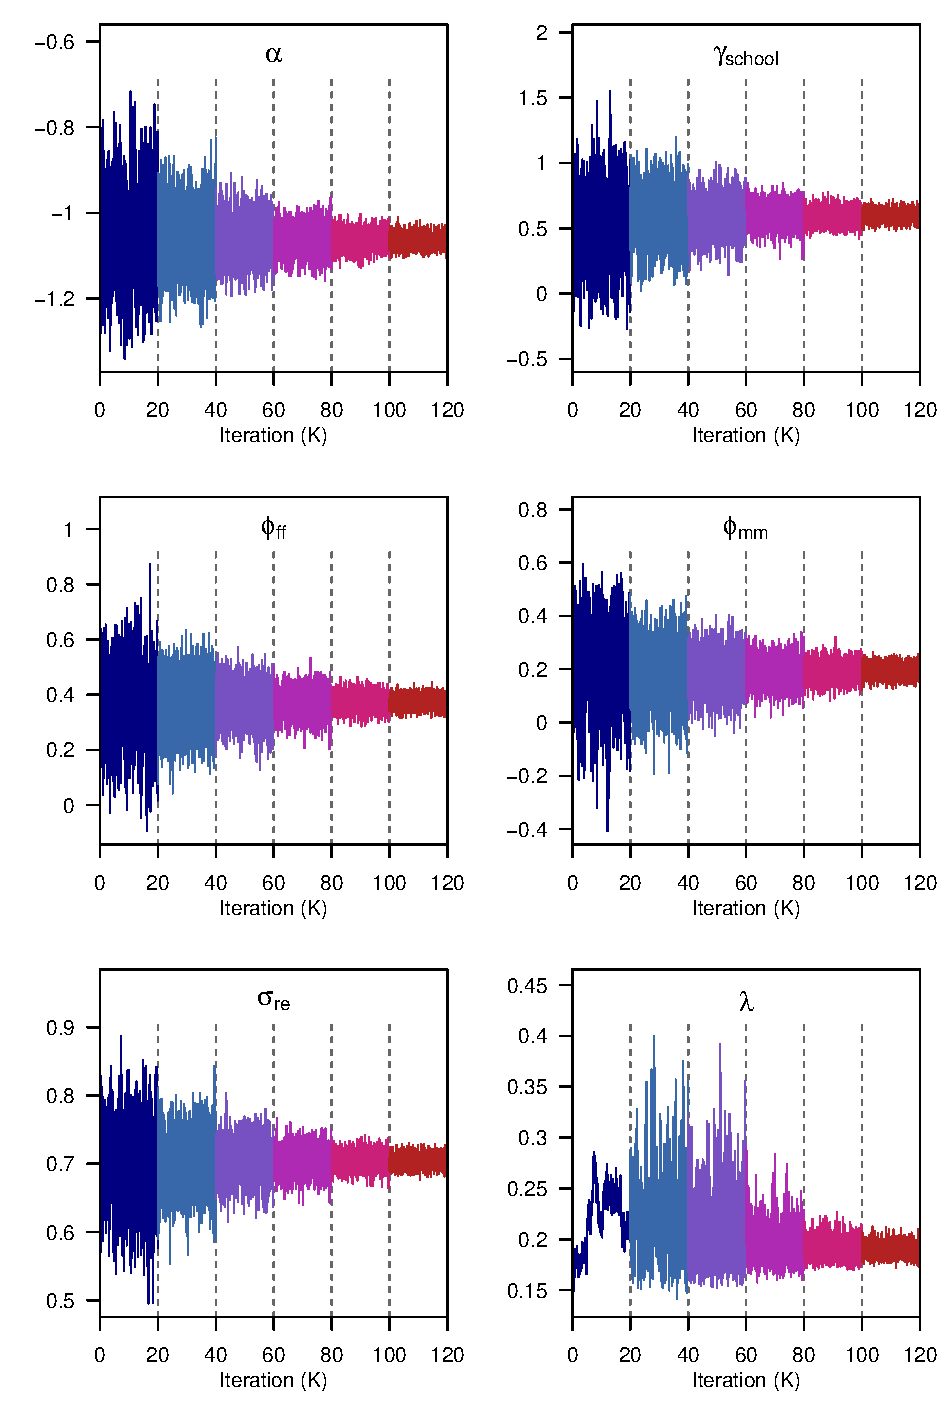
\includegraphics[width=0.75\textwidth]{figures/06_Appendix/model2a_multistage_traceplot_1.pdf}
\end{figure}
\begin{figure}[htbp]
    \centering
    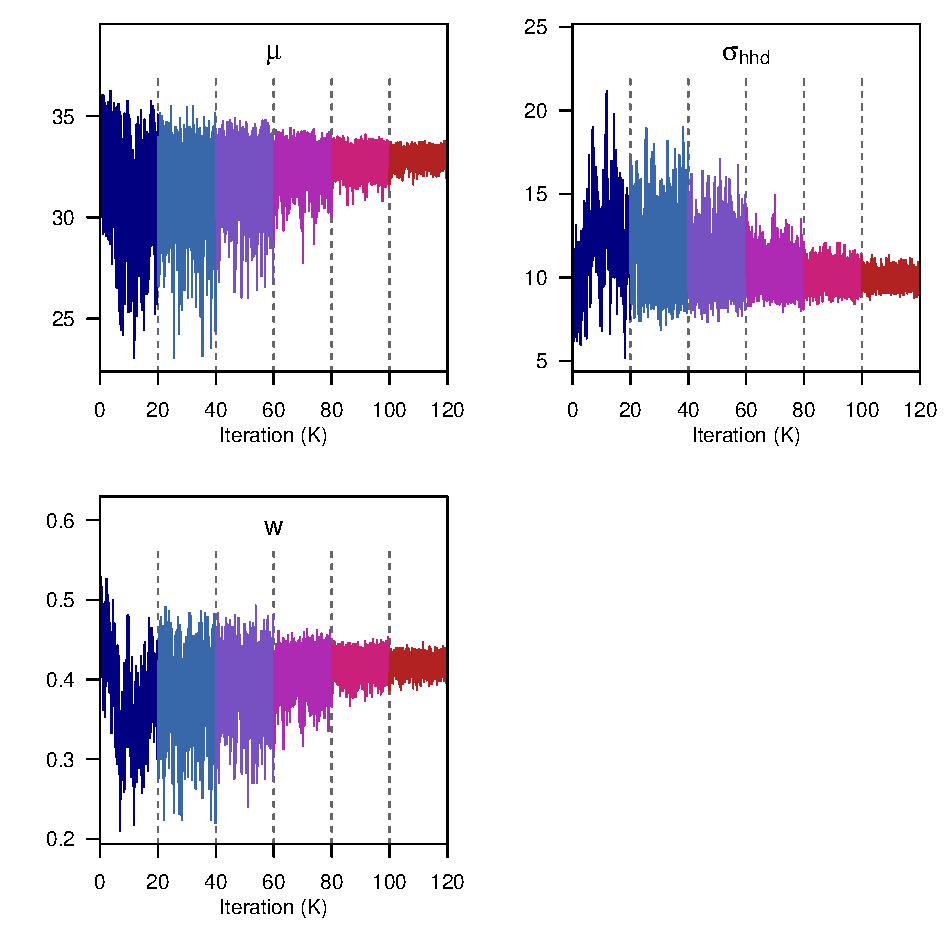
\includegraphics[width=0.75\textwidth]{figures/06_Appendix/model2a_multistage_traceplot_2.pdf}
    \caption{Model 2A: Multistage MCMC trace plots (Set 1 and 2).}
    \label{fig:trace_m2a_multi}
\end{figure}


\begin{figure}[htbp]
    \centering
    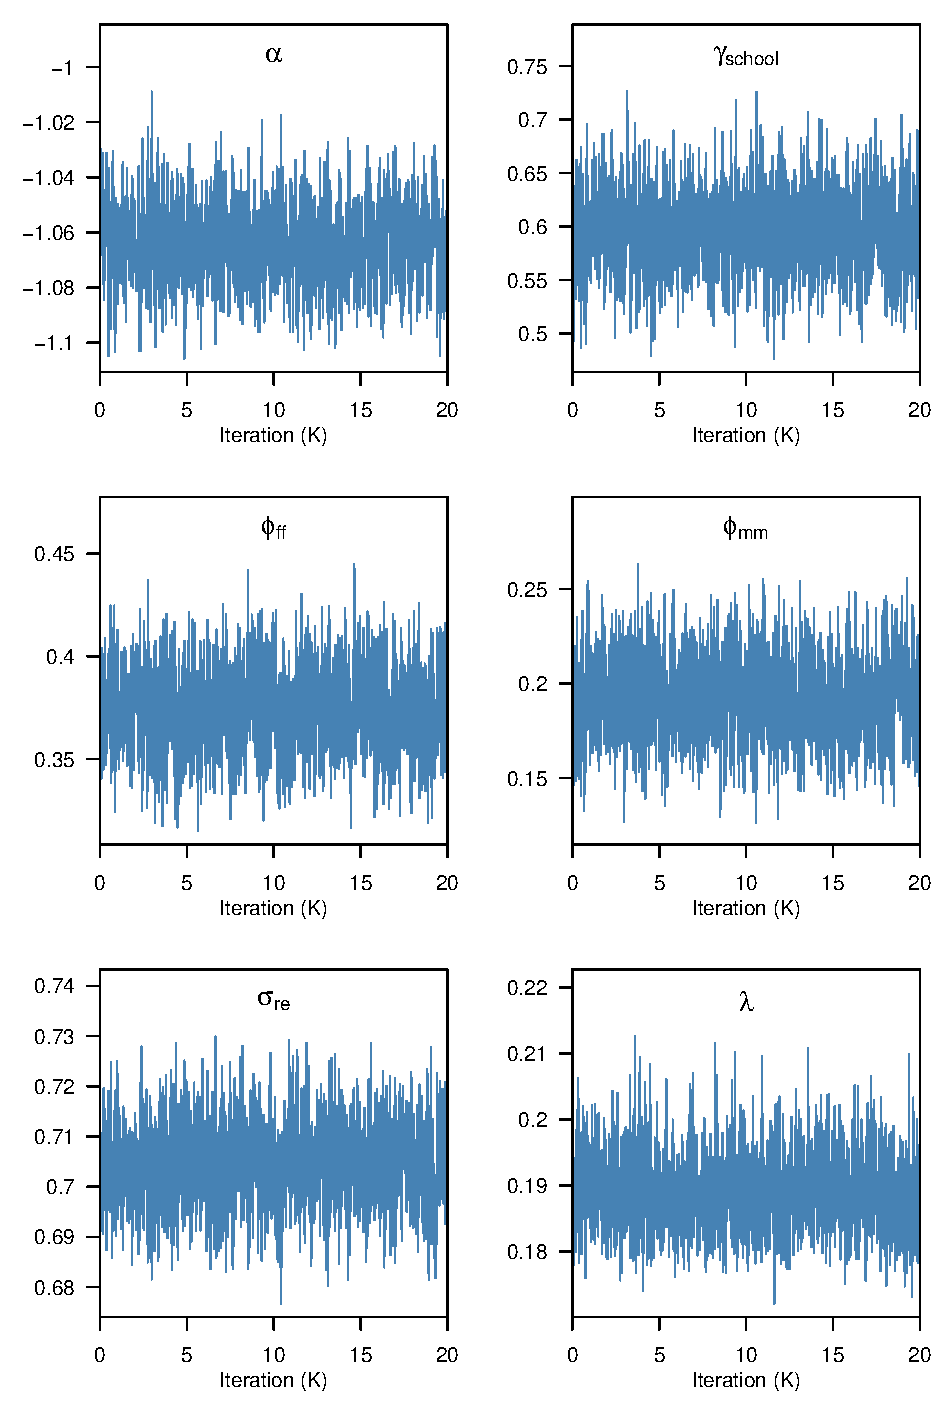
\includegraphics[width=0.75\textwidth]{figures/06_Appendix/model2a_singlestage_traceplot_1.pdf}
\end{figure}
\begin{figure}[htbp]
    \centering
    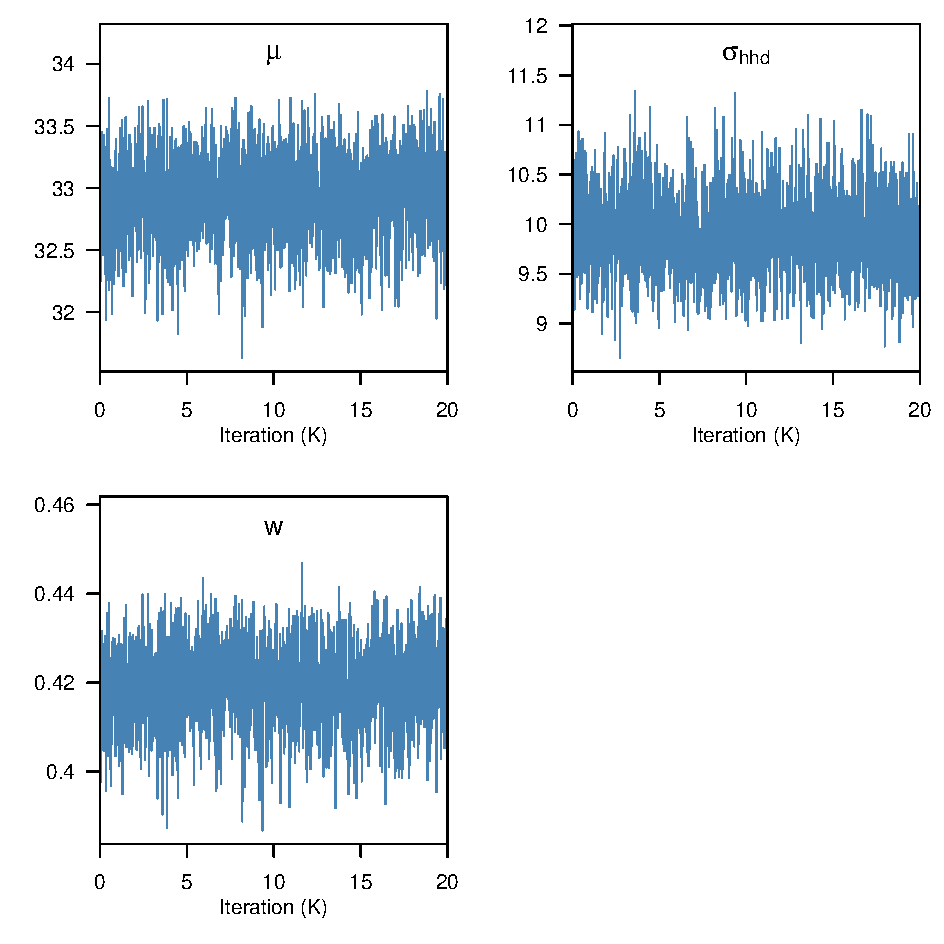
\includegraphics[width=0.75\textwidth]{figures/06_Appendix/model2a_singlestage_traceplot_2.pdf}
    \caption{Model 2A: Singlestage MCMC trace plots (Set 1 and 2).}
    \label{fig:trace_m2a_single}
\end{figure}

\clearpage

% ==========================================
% Model 2B
% ==========================================
\subsection*{B.3 Model 2B}

\begin{figure}[htbp]
    \centering
    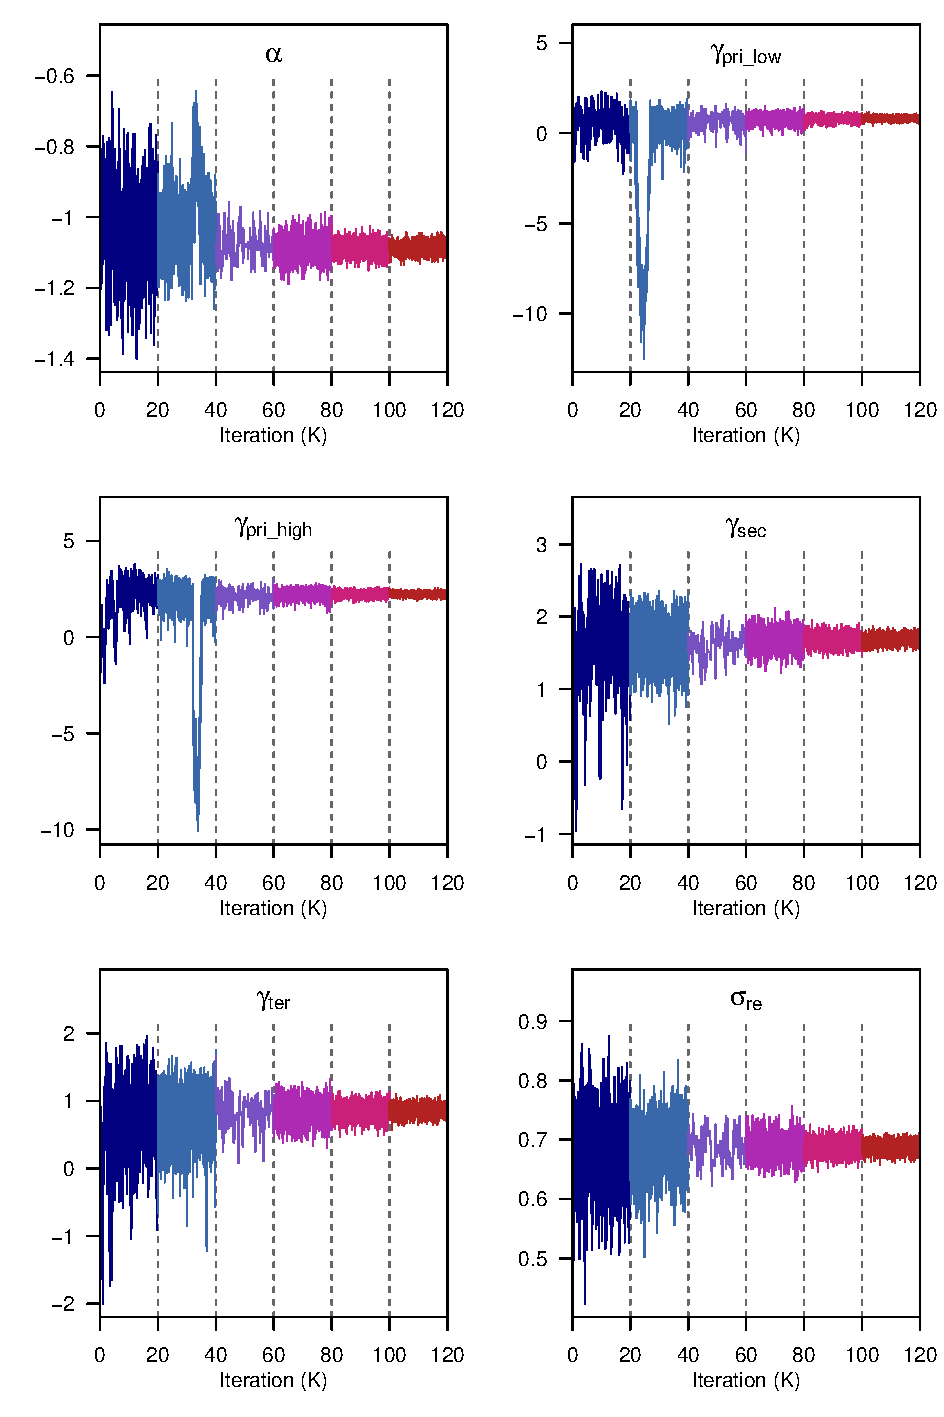
\includegraphics[width=0.75\textwidth]{figures/06_Appendix/model2b_multistage_traceplot_1.pdf}
\end{figure}
\begin{figure}[htbp]
    \centering
    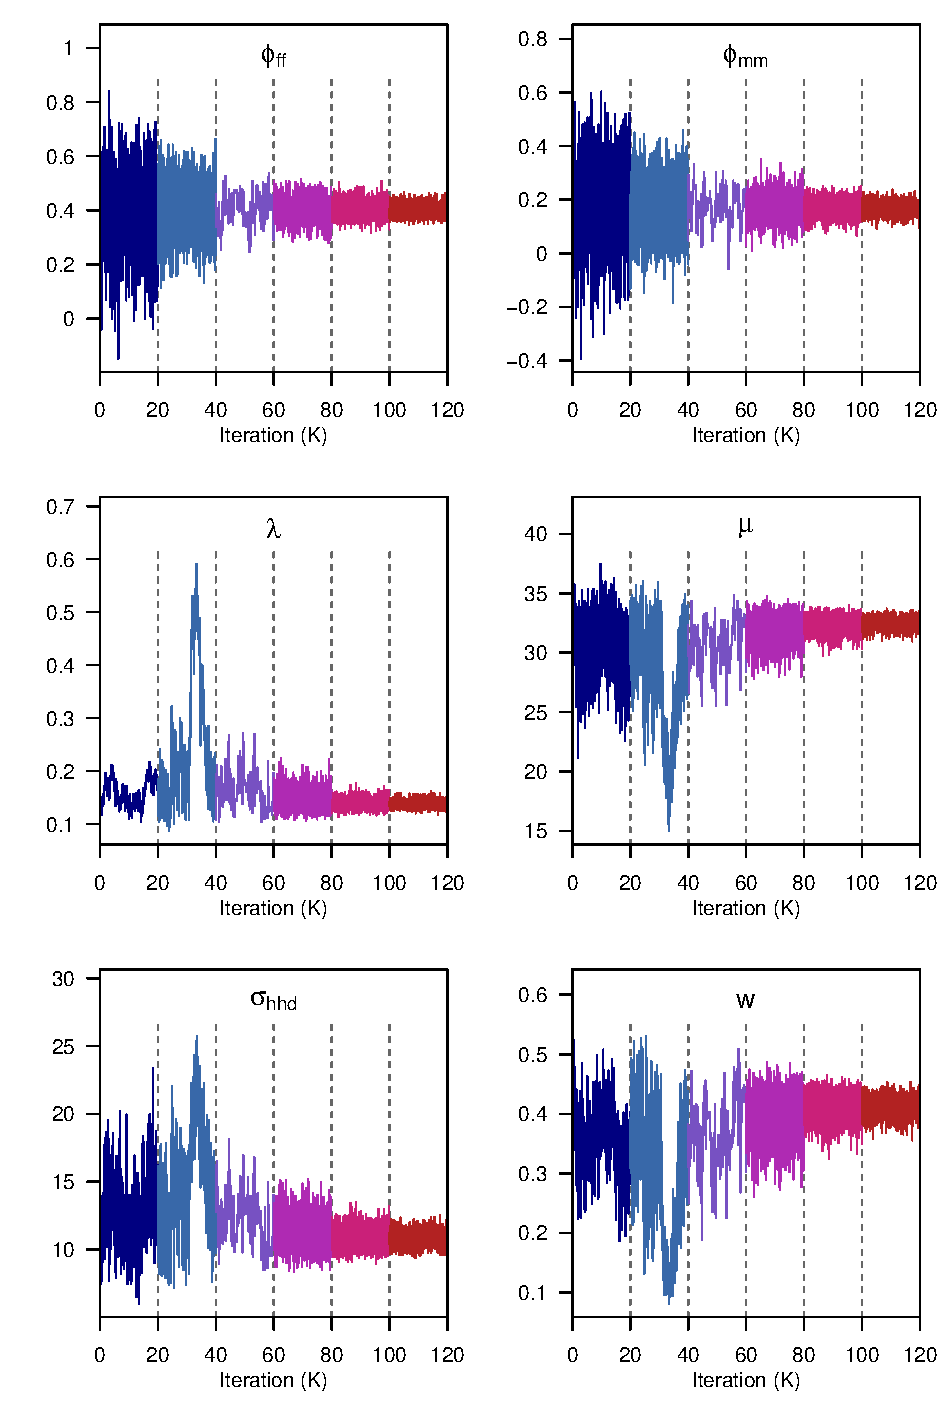
\includegraphics[width=0.75\textwidth]{figures/06_Appendix/model2b_multistage_traceplot_2.pdf}
    \caption{Model 2B: Multistage MCMC trace plots (Set 1 and 2).}
    \label{fig:trace_m2b_multi}
\end{figure}

\begin{figure}[htbp]
    \centering
    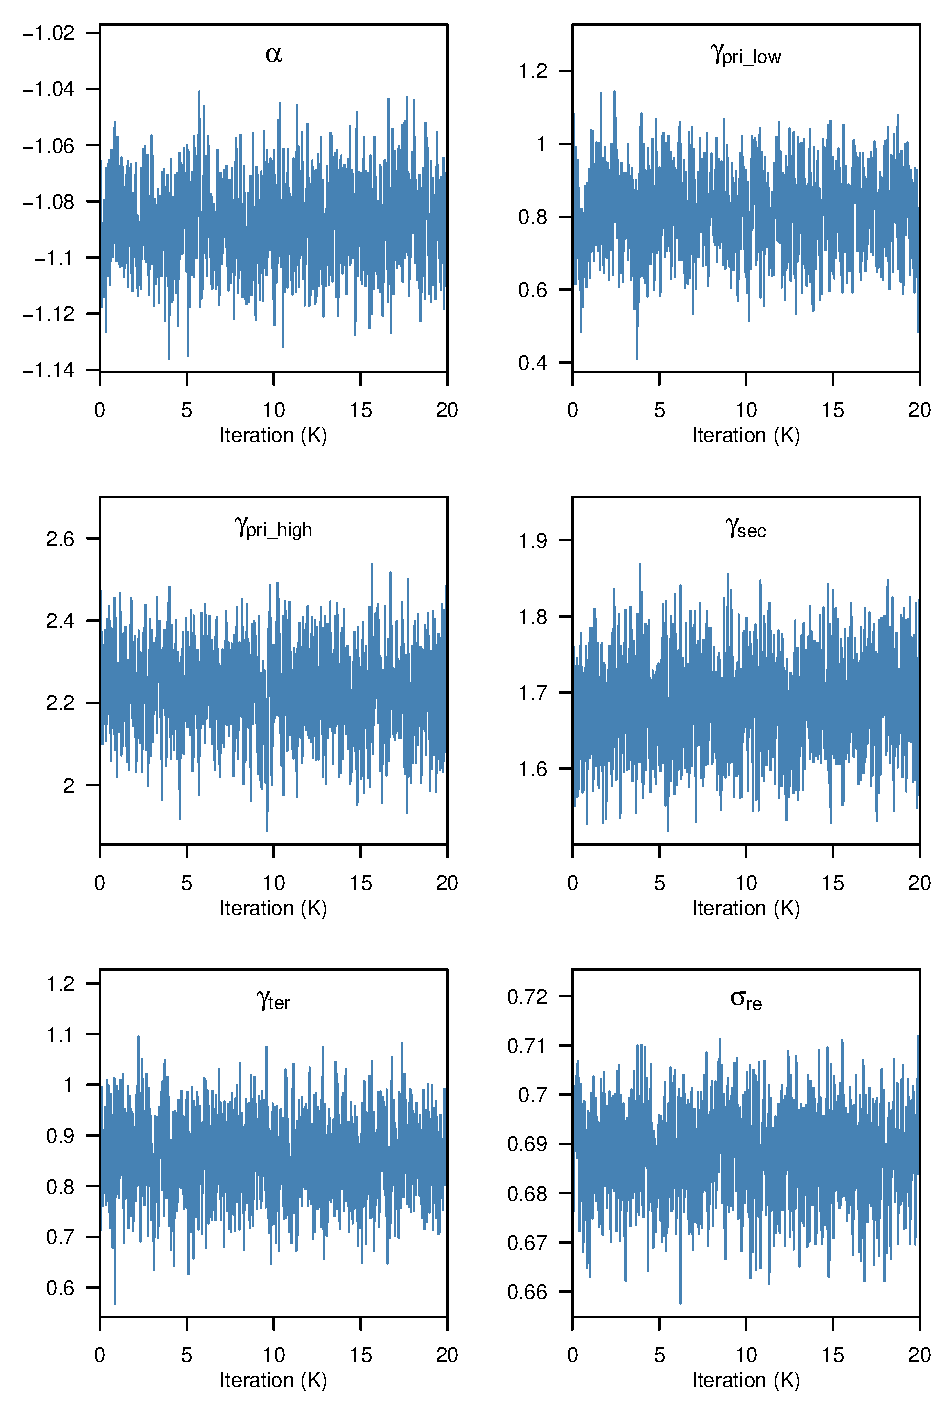
\includegraphics[width=0.75\textwidth]{figures/06_Appendix/model2b_singlestage_traceplot_1.pdf}
\end{figure}
\begin{figure}[htbp]
    \centering
    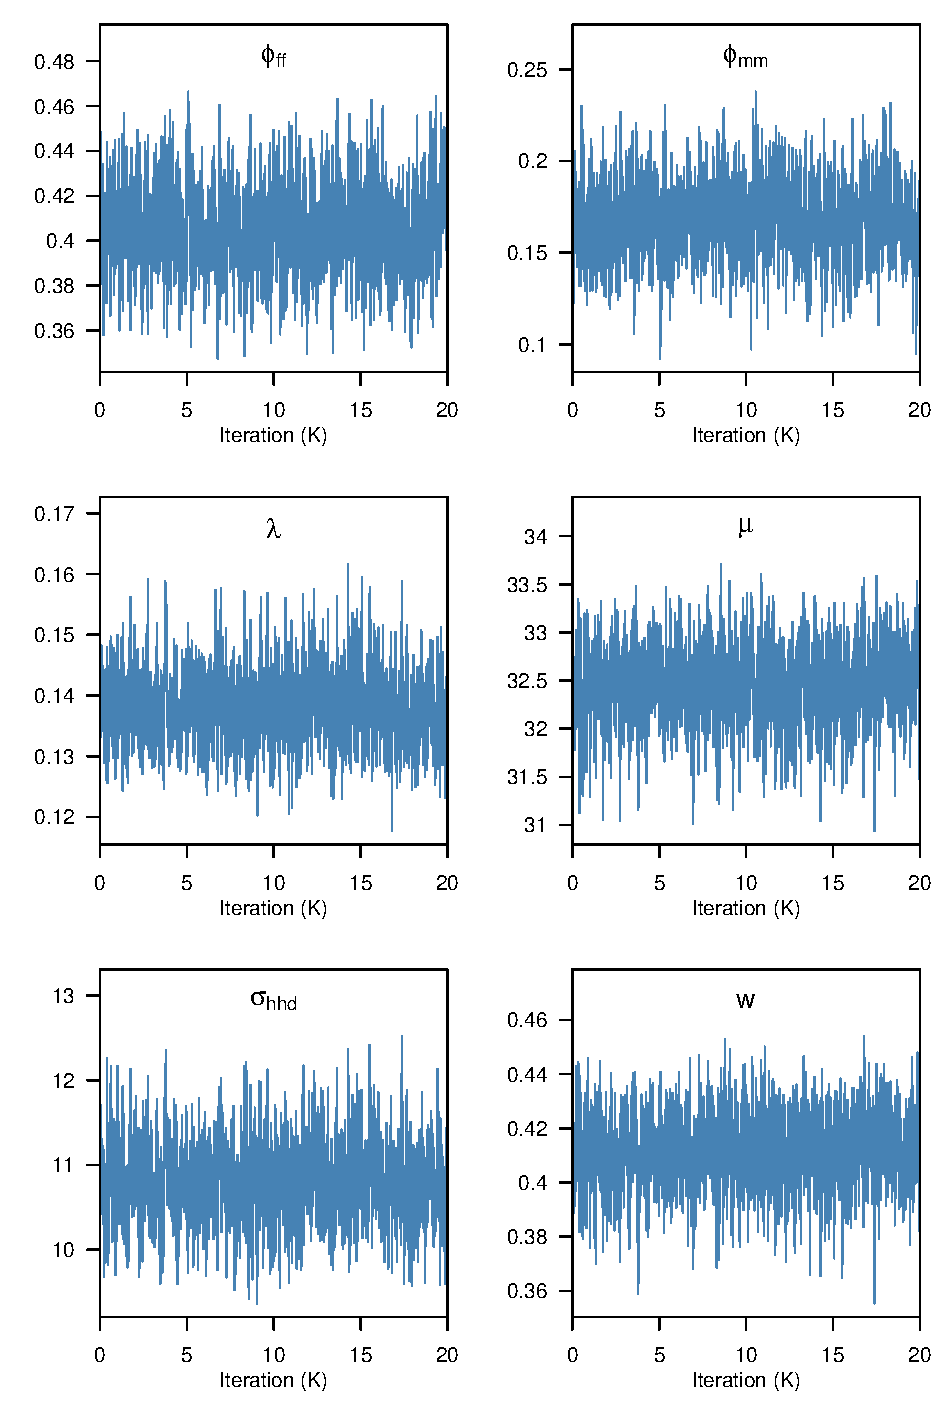
\includegraphics[width=0.75\textwidth]{figures/06_Appendix/model2b_singlestage_traceplot_2.pdf}
    \caption{Model 2B: Singlestage MCMC trace plots (Set 1 and 2).}
    \label{fig:trace_m2b_single}
\end{figure}

\clearpage


\section*{Appendix: Comparison of Summary Statistics}
\label{sec:appendix_stats_comparison}


% ==========================================
% Model 1
% ==========================================
\subsection*{C.1 Model 1: Summary Statistics Comparison}

\begin{table}[htbp]
    \centering
    \caption{Comparison of summary statistics for Model 1 (Base Model). The Z-score measures the deviation of the target from the simulation mean in units of simulation standard deviation.}
    \label{tab:stats_m1}
    \small
    \begin{tabular}{lcccccc}
        \toprule
        Statistic & Target Mean & Sim Mean & Z-Score & Sim 95\% Lower & Sim 95\% Upper \\
        \midrule
        Mean Degree   & 13.535 & 13.667 & -0.129 & 11.905 & 16.005 \\
        Log Variance  & 4.721  & 4.746  & -0.127 & 4.398  & 5.157 \\
        Mean Age Diff & 15.169 & 15.160 & 0.030  & 14.633 & 15.709 \\
        Prop MM       & 0.261  & 0.260  & 0.059  & 0.222  & 0.296 \\
        Prop FF       & 0.304  & 0.306  & -0.098 & 0.267  & 0.348 \\
        \bottomrule
    \end{tabular}
\end{table}

% ==========================================
% Model 2A
% ==========================================
\subsection*{C.2 Model 2A: Summary Statistics Comparison}

\begin{table}[htbp]
    \centering
    \caption{Comparison of summary statistics for Model 2A (Matrix model v4.2).}
    \label{tab:stats_m2a}
    \small
    \begin{tabular}{lcccccc}
        \toprule
        Statistic & Target Mean & Sim Mean & Z-Score & Sim 95\% Lower & Sim 95\% Upper \\
        \midrule
        Log Mean Degree      & 2.605 & 2.587 & 2.600 & 2.574 & 2.600 \\
        Prop Degree $\le$ 2  & 0.051 & 0.060 & -5.312 & 0.057 & 0.064 \\
        Prop Degree $\ge$ 25 & 0.148 & 0.117 & 13.591 & 0.113 & 0.121 \\
        Prop MM              & 0.261 & 0.265 & -0.856 & 0.256 & 0.273 \\
        Prop FF              & 0.304 & 0.301 & 0.499 & 0.293 & 0.310 \\
        Prop Age 0-5         & 0.410 & 0.410 & -0.050 & 0.403 & 0.417 \\
        Prop Age 6-15        & 0.186 & 0.185 & 0.182 & 0.181 & 0.190 \\
        Prop Age 20-35       & 0.245 & 0.235 & 4.019 & 0.231 & 0.240 \\
        Prop Age $> 40$      & 0.072 & 0.067 & 2.971 & 0.063 & 0.070 \\
        Prop School          & 0.223 & 0.223 & -0.022 & 0.213 & 0.233 \\
        \bottomrule
    \end{tabular}
\end{table}

\clearpage

% ==========================================
% Model 2B
% ==========================================
\subsection*{C.3 Model 2B: Summary Statistics Comparison}

\begin{table}[htbp]
    \centering
    \caption{Comparison of summary statistics for Model 2B (Refined school structure).}
    \label{tab:stats_m2b}
    \footnotesize
    \begin{tabular}{lcccccc}
        \toprule
        Statistic & Target Mean & Sim Mean & Z-Score & Sim 95\% Lower & Sim 95\% Upper \\
        \midrule
        Log Mean Degree      & 2.605 & 2.592 & 1.898 & 2.577 & 2.606 \\
        Prop Degree $\le$ 2  & 0.051 & 0.059 & -4.338 & 0.055 & 0.062 \\
        Prop Degree $\ge$ 25 & 0.148 & 0.123 & 11.262 & 0.118 & 0.127 \\
        Prop MM              & 0.261 & 0.259 & 0.284 & 0.250 & 0.269 \\
        Prop FF              & 0.304 & 0.307 & -0.765 & 0.298 & 0.316 \\
        Prop Age 0-5         & 0.410 & 0.412 & -0.554 & 0.405 & 0.419 \\
        Prop Age 6-15        & 0.186 & 0.184 & 0.813 & 0.179 & 0.188 \\
        Prop Age 20-35       & 0.245 & 0.232 & 5.534 & 0.227 & 0.236 \\
        Prop Age $> 40$      & 0.072 & 0.065 & 3.575 & 0.062 & 0.069 \\
        Prop Primary Low     & 0.028 & 0.025 & 1.653 & 0.021 & 0.029 \\
        Prop Primary High    & 0.045 & 0.042 & 0.792 & 0.037 & 0.048 \\
        Prop Secondary       & 0.097 & 0.102 & -1.457 & 0.095 & 0.109 \\
        Prop Tertiary        & 0.031 & 0.032 & -0.374 & 0.029 & 0.035 \\
        \bottomrule
    \end{tabular}
\end{table}

\end{document}